%% Based on a TeXnicCenter-Template by Tino Weinkauf.
%%%%%%%%%%%%%%%%%%%%%%%%%%%%%%%%%%%%%%%%%%%%%%%%%%%%%%%%%%%%%

%% Para arreglar el error que da el ifpdf
%% Sacado de internet:
%% Yes, \ifpdf is defined both in the class file and in the package ifpdf that is loaded by graphics.cfg. Workaround:
%%  \RequirePackage{ifpdf}
%%  \documentclass{JHEP3}
%% Then \ifpdf will be overwritten by the class, but with a similar meaning (the class is wrong for negative numbers of \pdfoutput). But the warning of ifpdf is not triggered and the package will not be loaded again later, because the package is already loaded.
\RequirePackage{ifpdf}

%%%%%%%%%%%%%%%%%%%%%%%%%%%%%%%%%%%%%%%%%%%%%%%%%%%%%%%%%%%%%
%% HEADER
%%%%%%%%%%%%%%%%%%%%%%%%%%%%%%%%%%%%%%%%%%%%%%%%%%%%%%%%%%%%%
\documentclass[a4paper,oneside,12pt]{report}
% Alternative Options:
%	Paper Size: a4paper / a5paper / b5paper / letterpaper / legalpaper / executivepaper
% Duplex: oneside / twoside
% Base Font Size: 10pt / 11pt / 12pt

%% Normal LaTeX or pdfLaTeX? %%%%%%%%%%%%%%%%%%%%%%%%%%%%%%%%
%% ==> The new if-Command "\ifpdf" will be used at some
%% ==> places to ensure the compatibility between
%% ==> LaTeX and pdfLaTeX.
\newif\ifpdf
\ifx\pdfoutput\undefined
	\pdffalse              %%normal LaTeX is executed
\else
	\pdfoutput=1           
	\pdftrue               %%pdfLaTeX is executed
\fi


%% Fonts for pdfLaTeX %%%%%%%%%%%%%%%%%%%%%%%%%%%%%%%%%%%%%%%
%% ==> Only needed, if cm-super-fonts are not installed
%\ifpdf
	%\usepackage{ae}       %%Use only just one of these packages:
	%\usepackage{zefonts}  %%depends on your installation.
%\else
	%%Normal LaTeX - no special packages for fonts required
%\fi


%% Language %%%%%%%%%%%%%%%%%%%%%%%%%%%%%%%%%%%%%%%%%%%%%%%%%
\usepackage[spanish]{babel}
\usepackage[T1]{fontenc}
\usepackage[latin1]{inputenc}


%% Packages for Graphics & Figures %%%%%%%%%%%%%%%%%%%%%%%%%%
\ifpdf %%Inclusion of graphics via \includegraphics{file}
	\usepackage[pdftex]{graphicx} %%graphics in pdfLaTeX
\else
	\usepackage[dvips]{graphicx} %%graphics and normal LaTeX
\fi
%\usepackage[hang,tight,raggedright]{subfigure} %%Subfigures inside a figure
%\usepackage{pst-all} %%PSTricks - not useable with pdfLaTeX


%% Math Packages %%%%%%%%%%%%%%%%%%%%%%%%%%%%%%%%%%%%%%%%%%%%
\usepackage{amsmath}
\usepackage{amsthm}
\usepackage{amsfonts}

%% Lists packages %%%%%%%%%%%%%%%%%%%%%%%%%%%%%%%%%%%%%%%%%%%
\usepackage{enumerate}
%\usepackage[shortlabels]{enumitem}


%% Line Spacing %%%%%%%%%%%%%%%%%%%%%%%%%%%%%%%%%%%%%%%%%%%%%
\usepackage{setspace}
%\singlespacing        %% 1-spacing (default)
\onehalfspacing       %% 1,5-spacing
%\doublespacing        %% 2-spacing


%% Other Packages %%%%%%%%%%%%%%%%%%%%%%%%%%%%%%%%%%%%%%%%%%%
%\usepackage{a4wide} %%Smaller margins = more text per page.
\usepackage{fancyhdr} %%Fancy headings
\usepackage{longtable} %%For tables, that exceed one page
\usepackage{rotating} %%permite rotar tablas
\usepackage{multirow} %% permite tener multilineas en una tabla

\usepackage{wrapfig}

%%\usepackage{tex4ht}
%%%%%%%%%%%%%%%%%%%%%%%%%%%%%%%%%%%%%%%%%%%%%%%%%%%%%%%%%%%%%
%% Remarks
%%%%%%%%%%%%%%%%%%%%%%%%%%%%%%%%%%%%%%%%%%%%%%%%%%%%%%%%%%%%%
%
% TODO:
% 1. Edit the used packages and their options (see above).
% 2. If you want, add a BibTeX-File to the project
%    (e.g., 'literature.bib').
% 3. Happy TeXing!
%
%%%%%%%%%%%%%%%%%%%%%%%%%%%%%%%%%%%%%%%%%%%%%%%%%%%%%%%%%%%%%

%%%%%%%%%%%%%%%%%%%%%%%%%%%%%%%%%%%%%%%%%%%%%%%%%%%%%%%%%%%%%
%% Options / Modifications
%%%%%%%%%%%%%%%%%%%%%%%%%%%%%%%%%%%%%%%%%%%%%%%%%%%%%%%%%%%%%

%\input{options} %You need a file 'options.tex' for this
%% ==> TeXnicCenter supplies some possible option files
%% ==> with its templates (File | New from Template...).

%% MARCADEAGUA
%%%%%%%%%%%%%%%%%%%%%%%%%%%%%%%%%%%%%%%%%%%%%%%%%%%%%%%%%%%%%
%% Marca de agua (mientras se escribe el documento)
%%%%%%%%%%%%%%%%%%%%%%%%%%%%%%%%%%%%%%%%%%%%%%%%%%%%%%%%%%%%%

%% C�digo para poner una marca de agua mientras escribimos el documento.
%% Recomiendo buscar el tag MARCADEAGUA por el documento para ver d�nde se usa.

%\usepackage{eso-pic}
%\newcommand\BackgroundPic{
	%\put(0,0){
		%\parbox[b][\paperheight]{\paperwidth}{
			%\vfill
			%\centering
			%
\includegraphics[width=\paperwidth, height=\paperheight, keepaspectratio]{imgs/marcadeagua_endesarrollo.png}
			%\vfill
		%}
	%}
%}
%% FIN MARCADEAGUA
\usepackage{wallpaper}


%% Links en la tabla de contenidos
%\usepackage[linktoc=all]{hyperref}
%\setcounter{secnumdepth}{0}
%\usepackage{titlesec}
%\hypersetup{
    %colorlinks,
    %citecolor=black,
    %filecolor=black,
    %linkcolor=black,
    %urlcolor=black
%}

%%%%%%%%%%%%%%%%%%%%%%%%%%%%%%%%%%%%%%%%%%%%%%%%%%%%%%%%%%%%%
%% DOCUMENT
%%%%%%%%%%%%%%%%%%%%%%%%%%%%%%%%%%%%%%%%%%%%%%%%%%%%%%%%%%%%%
\begin{document}

%% MARCADEAGUA
%\AddToShipoutPicture{\BackgroundPic}
\ULCornerWallPaper{1}{imgs/marcadeagua_endesarrollo.png}
%% FIN MARCADEAGUA

%% File Extensions of Graphics %%%%%%%%%%%%%%%%%%%%%%%%%%%%%%
%% ==> This enables you to omit the file extension of a graphic.
%% ==> "\includegraphics{title.eps}" becomes "\includegraphics{title}".
%% ==> If you create 2 graphics with same content (but different file types)
%% ==> "title.eps" and "title.pdf", only the file processable by
%% ==> your compiler will be used.
%% ==> pdfLaTeX uses "title.pdf". LaTeX uses "title.eps".
\ifpdf
	\DeclareGraphicsExtensions{.pdf,.jpg,.png}
\else
	\DeclareGraphicsExtensions{.eps}
\fi

\pagestyle{fancy} %No headings for the first pages.


%% Title Page %%%%%%%%%%%%%%%%%%%%%%%%%%%%%%%%%%%%%%%%%%%%%%%
%% ==> Write your text here or include other files.

%% The simple version:
\begin{figure}
	\centering
		
\includegraphics[width=0.50\textwidth]{imgs/logo_usp_12star.jpg}
\end{figure}


\title{Aqu� va el nombre del proyecto}
\author{Jos� Carlos Jim�nez G�mez}
%\date{7 de febrero de 2012} %%If commented, the current date is used.

\maketitle
 

%% The nice version:
%%% Based on a TeXnicCenter-Template by Tino Weinkauf.
%%%%%%%%%%%%%%%%%%%%%%%%%%%%%%%%%%%%%%%%%%%%%%%%%%%%%%%%%%%%%

%%%%%%%%%%%%%%%%%%%%%%%%%%%%%%%%%%%%%%%%%%%%%%%%%%%%%%%%%%%%%
%% Deckblatt
%%%%%%%%%%%%%%%%%%%%%%%%%%%%%%%%%%%%%%%%%%%%%%%%%%%%%%%%%%%%%
%%
%% ATTENTION: You need a main file to use this one here.
%%            Use the command "\input{filename}" in your
%%            main file to include this file.
%%

%% Definici�n de autor, t�tulo y fecha para reutilizar
\author{Jos� Carlos Jim�nez G�mez}
\title{<T�TULO DEL\\
PROYECTO FINAL DE CARRERA>}
\date{\today}
%\newdateformat{mydate}{\monthname[\THEMONTH] \THEYEAR} 
%http://www.howtotex.com/packages/customize-the-date-format-in-your-latex-documents/#sthash.rmRWrHms.dpuf

\makeatletter	%% Para poder usar las definiciones anteriores. Hay que cerrar con \makeatother

\begin{titlepage}
\begin{center}

\Large
\vspace{1cm}
\textsf{UNIVERSIDAD SAN PABLO - CEU\\}
\vspace{1cm}
\large
\textsf{ESCUELA POLIT�CNICA SUPERIOR\\}
\vspace{2cm}
\textsf{INGENIER�A INFORM�TICA\\}
\vspace{2cm}

\begin{figure}[htbp]
	\centering
		
\includegraphics[width=0.30\textwidth]{imgs/logoceu.jpg}
		%
\includegraphics[width=0.50\textwidth]{imgs/logo_usp_12star.jpg}
	\label{fig:logoceu}
\end{figure}
%\begin{figure}
	%\centering
		%
\includegraphics[width=0.50\textwidth]{imgs/logo_usp_12star.jpg}
%\end{figure}

\large
\vspace*{2cm}
\textsf{PROYECTO FINAL DE CARRERA\\}

\Large
\vspace*{1cm}
\textsf{\@title}
\vspace{1cm}

\large
\textsf{Autor: \@author\\
Director: Ra�l Garc�a Garc�a}
\vspace{1cm}


%\textsf{Enero 2008}\\ %%Date - better you write it yourself.
\textsf{\date{\today}}\\ %%Date - better you write it yourself.
\date{\today}

\@date


\end{center}

\end{titlepage}

\makeatother	%% Necesario este ''cierre'' para el \makeatletter para poder usar las referencias a title, author y date
 %%You need a file 'titlepage.tex' for this.
%% ==> TeXnicCenter supplies a possible titlepage file
%% ==> with its templates (File | New from Template...).



%% Introducci�n %%%%%%%%%%%%%%%%%%%%%%%%%%%%%%%%%%%%%%%

\chapter*{Agradecimientos}
\addcontentsline{toc}{chapter}{Agradecimientos}
\par

Hay demasiadas personas a las que debo agradecer que este PFC se haya redactado y haya obtenido la carrera de Ingenier�a Inform�tica. Aqu� lo que quiero es agradecer a algunas de ellas que creo que merecen formar parte de este documento. \\

En primer lugar quiero dar las gracias a mis padres y a mi hermana Marta, mi familia. Sin ellos, sin su ayuda, sin su apoyo, este proyecto no ser�a posible. Para ellos es cada una de las p�ginas e ideas aqu� plasmadas. \\

A Bego�a. Ella es la que ha tenido que soportar todo lo que este proyecto ha conllevado. Gracias por aguantarme, sobre todo mi car�cter, mi genio, mis divagaciones filos�ficas acerca del voto por Internet. Y, sobre todo, gracias por el tiempo que me has dado y todo aqu�l que no hemos aprovechado juntos por dedicarlo a este PFC. Espero poder devolv�rtelo a partir de ahora. \\

A la gente del Sanagus, en especial a mis compa�eros de piso Jordi, Dj y Molinete, que me han acompa�ado durante todos mis a�os universitarios. Gracias a Ana, que tambi�n tuvo que soportar bastante mi car�cter al inicio de esta aventura. Adem�s del tiempo que me dedicaste, valoro el que me hicieras aprobar Econom�a, si no es por ti... ;) Y a Felipe, que me ha dado su confianza y la oportunidad de ayudarle en su nueva aventura a la vez que �l me ayuda a adaptarme a los \textit{nuevos tiempos}. \\

A mis compa�eros y amigos de Indra, nombrando a David, Mariano, Jes�s, Fernando, Sara, Pedro, Elena, Luis, Rodrigo, Lorena, Juli�n, Zule, Cari, Eduardo, Bel�n... y podr�a seguir nombrando durante muchas l�neas. De casi todos he aprendido much�simo m�s de lo que he ense�ado, as� que el balance es positivo. Ha sido un placer compartir tiempo y conocimiento con el grupo de ingenieros m�s experto en elecciones que hay en este pa�s. \\

A mis compa�eros en la carrera, incluidos los miembros del Gang of Five. Carfes�n, Juaca, Weil, Marta, Chac�n, Kapi, Vendrell, Juanolo, Charly... tambi�n me faltan hojas para nombraros a todos. Fue un placer compartir estos a�os con vosotros. \\

A mis profesores, que son los que emplearon su tiempo y energ�a en que pudiese obtener los conocimientos necesarios para formarme como Ingeniero. \\

A mis primos, t�os y abuelos. Mi familia es grande, pero siempre hab�is estado ah�. Y los que falt�is, espero que pueda haceros sentir orgullosos con mi forma de ser. \\

Al Betis. Por el sufrimiento de cada semana. Por su bandera, que me ha dado un hobby viajero. Y por aquel junio de 2005. ;) Y a Iniesta, por aquel julio de 2010. \\

A Ram�n, por demasiadas cosas. Hace un tiempo aqu� habr�a puesto que gracias por ser  \textit{mi hermano mayor} y compa�ero de pr�cticas, estudio, fiestas y vida. Pero, junto con Mar�a, me hab�is \textit{presentado} a mis \textit{sobris} �ngel e Irene y todo ha cambiado. Ahora tengo que agradeceros todo a los cuatro, no a ti solo. Menos mal que siempre has estado ah�, que est�is ah�. \\

A Ra�l, mi tutor, por TODO. Literalmente, te debo que este PFC se haya llegado a presentar. Despu�s de tanto tiempo de charlas y emails creo que no he llegado a agradecerte suficientemente lo que has hecho por m�. Espero que no se quede corto resumirlo en dos simples palabras: Muchas gracias. \\

A todo los nombrados aqu� y a los que no, pero a�n as� deber�an estar, muchas gracias. Espero poder aportar a los dem�s todo lo que he recibido de vosotros. \\

Gracias.


\chapter*{Resumen}
\par
Con el creciente desarrollo de la tecnolog�a y su implantaci�n en la mayor�a de los campos de la vida cotidiana, es inevitable pensar en soluciones electr�nicas para un elemento tan importante de nuestra sociedad como son los procesos electorales.
\par 
Encontramos procesos electorales en multitud de organizaciones, desde estados nacionales a empresas privadas, pasando por juntas de administraciones u organismos p�blicos.
\par
En cambio, contrario a lo que puede parecer por el intenso uso de las nuevas tecnolog�as en campos como las transacciones bancarias, telemedicina, comunicaciones o gestiones con la Administraci�n, en el mundo electoral no se est� terminando de introducir el voto telem�tico a gran escala. De hecho, aunque encontramos algunas excepciones como pueden ser Estonia, Venezuela, Brasil y algunos territorios m�s reducidos, no se utiliza a estos niveles en la totalidad del proceso electoral, quedando reducido a algunas fases del proceso o, simplemente, a ninguna.
\par
En este PFC, vamos a evaluar la implantaci�n del voto telem�tico a peque�a escala para tratar de escalar los problemas que comportan a nivel nacional. Para ello, vamos a realizar un sistema que soportar� de forma �ntegra las elecciones a la Junta de Escuela de la Escuela Polit�cnica Superior de la Universidad San Pablo CEU.
\par
A partir de este desarrollo, trataremos de hacer frente, a peque�a escala, a los problemas que nos encontramos en estas grandes elecciones, aunque para ello tengamos que variar los requisitos ideales para la simple consecuci�n de la elecci�n que implementamos.

\chapter*{Abstract}
\par
El sistema actual de telemedicina de las Fuerzas Armadas en Espa�a, separa los distintos integrantes en cuatro roles, desde los de intervenci�n m�s r�pida (tales como veh�culos ambulancia blindados, pr�ximos a los nidos de heridos), a los de intervenci�n menos r�pida pero con mayor capacidad m�dica (hospitales de la infraestructura nacional).
\par 
En la actualidad, est� perfectamente resuelto todo lo relativo a los sistemas de intercambio de informaci�n y comunicaci�n de eventos entre los roles de niveles 3 y 4. La problem�tica de estos roles, ya resuelta, correspond�a con la capacidad de facilitar asistencia desde la infraestructura nacional a los puestos m�dicos fuera del territorio nacional.
\par
En cambio, a�n no se han creado sistemas para solucionar las problem�ticas existentes en los roles 1 y 2, donde las unidades se encuentran en zonas m�s desplazadas, con menos medios, pero con mayor velocidad de actuaci�n.
\par
El objetivo de este proyecto es aportar soluciones para las problem�ticas planteadas en estos roles 1 y 2.
\chapter{Introducci�n}
	\rhead{Introducci�n}
	\par
	Este proyecto trata de entrar en la problem�tica del voto electr�nico remoto frente al presencial, de las reticencias sociales y tecnol�gicas que influyen en su reducida implantaci�n en procesos electorales de gran importancia y alto n�mero de electores. Para ello, vamos a reproducir la situaci�n a escala reducida. Plantearemos una posible soluci�n al proceso necesario para llevar a cabo las Elecciones a la Junta de Escuela de la Escuela Polit�cnica Superior de la Universidad San Pablo - CEU.
	\par
	Con este planteamiento es obvio que no vamos a solucionar las trabas t�cnicas y sociales del voto por internet a nivel de unas elecciones legislativas en, por ejemplo, Espa�a. Es un tema que se escapa del objetivo de este PFC, pero s� que vamos a tratar de identificar algunos de los agentes influyentes y buscar una posible soluci�n aplicable a la elecci�n a la Junta de Escuela.
	\par
	As�, conseguiremos dos objetivos. Por un lado, estudiar la dificultad existente para la implantaci�n del voto por internet en las elecciones nacionales. Por otro, un soporte electr�nico al proceso completo de las Elecciones a la Junta de Escuela, con el cual obtendremos una mejora significativa en el mismo respecto a procesos anteriores.
	\par
	Antes de entrar en detalle en el proceso, habr� que definir el tipo de votaci�n que queremos implementar. No se habla en este PFC de voto electr�nico como tal, ni siquiera de voto electr�nico remoto. Lo que se quiere implementar es una soluci�n de voto por internet, en el que no haga falta la presencia f�sica del votante en el centro de votaci�n, que tenga la oportunidad de ejercer su derecho al voto desde cualquier punto del planeta con conexi�n a internet. Este detalle, que puede parecer trivial al querer separarlo del concepto de voto electr�nico, en realidad es fundamental. En un pr�ximo cap�tulo se ahondar� en ello, pero podemos avanzar que una de las grandes diferencias a tener en cuenta es que con voto electr�nico remoto, podemos utilizar m�quinas de votaci�n (que tambi�n emitir�an el voto por internet), las cuales pueden generar un recibo con el voto emitido por el votante, al estilo de las papeletas que llenan la urna electoral, mientras que con el voto por internet puro, esto no es tan obvio. Con este mecanismo, la auditor�a es m�s simple para el voto electr�nico con m�quinas en el centro de votaci�n, pues se podr�an contar las papeletas generadas. �Qu� ocurre con el voto por internet, en el que no se generan estos recibos ni hay una urna f�sica donde se depositan? �Qu� ocurre si el sistema tiene fallas y no se contabilizan (o lo hacen de forma incorrecta) los sufragios, teniendo en cuenta que puede ser imposible un conteo f�sico de papeletas al no existir estas? Como estas, hay muchas cuestiones a las que el voto por internet debe dar soluci�n de forma fiable antes de poder acometer su implantaci�n en procesos electorales de envergadura e importancia.
	\par
	La forma de llegar a la soluci�n buscada debe comenzar identificando los factores que afectan a un proceso electoral general y, a continuaci�n, personalizar los que se encuentran en el que vamos a estudiar.
	Una vez identificados estos agentes, definiremos las fases que comportan unas elecciones y estudiaremos c�mo podr�an ser apoyadas tecnol�gicamente, evaluando c�mo llegar al punto �ptimo de integraci�n con el sistema tradicional para mejorar el proceso.
	\par
	La primera fase se concentrar� en desarrollar los sistemas asociados a la fase preelectoral. En ella, se recoge el censo electoral y se identifican tanto los candidatos como los diferentes cargos que se votan.
	%%OJO: �hay que hablar de la l�gica de la elecci�n? De c�mo se vota y qui�n para elegir el qu� y c�mo??
	\par
	La segunda fase, la electoral, la identificamos con los procesos que se requieren durante el periodo que dura la elecci�n (ya sea un d�a o varios). Esta consistir� en desarrollar los sistemas de identificaci�n y validaci�n de votantes, el sistema de votaci�n, ss


	\section{Motivaci�n del Proyecto}\label{motivacion}
		%El Proyecto Fin de Carrera que presento consiste en el dise�o e implementaci�n de un sistema de voto por internet para dos elecciones de la Escuela Polit�cnica Superior de la Universidad San Pablo CEU.\\
		%Desde que sal� de la Escuela y comenc� a desempe�arme profesionalmente, el sector en el que me he ubicado ha sido el de los Procesos Electorales. En este, he desarrollado, sobre todo, software orientado a la difusi�n de resultados, aunque adem�s he participado en un sistema de Atenci�n a Usuarios de dispositivos de conteo electoral, un sistema de registro de electores previo a votaci�n y otros  proyectos diversos.\\
		%Despu�s de tanto tiempo en el sector es invitable mantener conversaciones acerca de las elecciones, los sistemas de informaci�n que se usan, los que podr�an usarse, los que se han denostado y los que se vislumbran para el futuro.\\
		%Una de estas conversaciones fue con un profesor de esta misma Escuela, unos d�as despu�s de las Elecciones Generales de 2012, en las que me coment� que hab�a probado un sistema piloto implementado para aqu�l comicio para el municipio de Madrid, el cual ten�a por nombre Mesa Administrada Electr�nicamente. Hablamos de que usando su DNIe, se identific� ante el Presidente de la Mesa Electoral y, a trav�s de un port�til, se le encontr� en el censo, se le marc� como votado e, incluso, se le imprimi� un justificante de votaci�n. Todo esto en poco tiempo. Tras indagar lo que opinaba del sistema, me dijo que lo que realmente esperaba es que para las siguientes elecciones, ni siquiera tuviese que salir de casa, que pudiese votar desde all�, por internet.\\
		%Ese fue el germen de este PFC, la idea de encontrar una soluci�n viable al voto por internet. No obstante, este estudio, a nivel nacional, puede resultar muy extenso. Por ello, la idea vir� hacia la realizaci�n de un sistema m�s peque�o, como son unas elecciones en la Escuela, pero igual de ambicioso y escalable, buscando encontrar una primera piedra para construir un sistema robusto que pueda cubrir las necesidades funcionales, de seguridad y de confianza necesarias para unas elecciones a nivel estatal.\\
		%Siempre me llam� la atenci�n que, pese al ritmo de evoluci�n y progreso de los sistemas de informaci�n y las nuevas tecnolog�as en todos los �mbitos, en el electoral se segu�a ejerciendo el voto como cuando vot� por primera vez a los 18 a�os, igual incluso que la primera vez que recuerdo acompa�ar a mis padres cuando era mucho m�s joven. Otra motivaci�n, pues, es tratar de entender los motivos que hacen que el desarrollo tecnol�gico en este campo no parezca, a simple vista, evolucionar a la misma velocidad que en el resto de �mbitos cotidianos.\\
		********** COMENTADO POR AHORA ***************
		********** FALTA. �C�MO SE INDENTA CUANDO TAN S�LO HEMOS HECHO UN SALTO DE P�GINA ***************

	\section{Antecedentes}\label{antecedentes}
	El voto electr�nico se lleva tratando de desarrollar e implementar desde hace bastante tiempo. Concretamente, podr�amos datar el comienzo en el a�o 1868, cuando el inventor estadounidense Thomas Alva Edison (1847-1931) registr� su primera patente, consistente en un instrumento simple para el recuento mec�nico de votos. El instrumento se pod�a colocar en la mesa delante de cada congresista y ten�a dos botones, uno para el voto a favor y otro para el voto en contra. Pese a considerarlo un avance, no consigui� ser aceptado en el Congreso de Washington, donde le dieron el siguiente motivo para argumentar el rechazo de los representantes a esta nueva tecnolog�a: XXXXOJO "\textit{If there is any invention on Earth that we don't want down here, that is it.}" "\textit{Joven, si hay en la tierra alg�n invento que no queremos aqu�, es exactamente el suyo. Uno de nuestros principales intereses es evitar fraudes en las votaciones, y su aparato no har�a otra cosa que favorecerlos}".
	\begin{figure}[htbp]
		\centering
			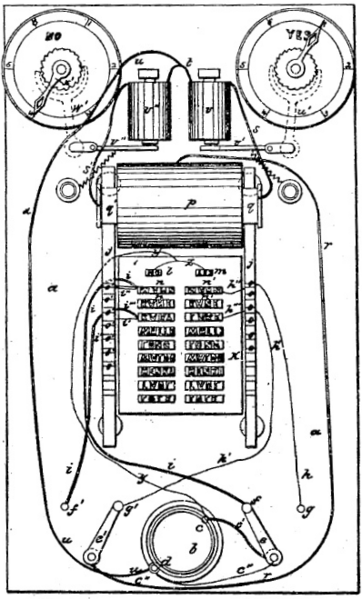
\includegraphics[width=0.30\textwidth]{imgs/Edisonsfirstpatent.png}
		\caption{U.S. Patent 0,090,646 -- Electrographic Vote-Recorder: Primera patente de Thomas A. Edison. Permit�a un voto de tipo 'A favor' o 'En contra' a trav�s de dos interruptores. (1869). Fuente: Wikipedia}
		\label{fig:primeraPatenteEdison}
	\end{figure}
	\begin{figure}[htbp]
		\centering
			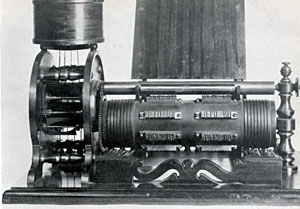
\includegraphics[width=0.30\textwidth]{imgs/EdisonVotingRecorder.jpg}
		\caption{Electrographic Vote-Recorder: Fotograf�a del invento de Thomas A. Edison. Fuente: Rutgers.edu}
		\label{fig:maquinaVotacionEdison}
	\end{figure}
	

	\par
	A partir de este intento, el voto electr�nico ha avanzado tecnol�gica y socialmente, logrando herramientas m�s sofisticadas y seguras en conjunci�n con un entendimiento, comprensi�n y, en algunos casos, aceptaci�n de su uso. Estos factores han hecho posible que se hayan podido implementar soluciones e integrarlas en procesos electorales reales, ya sea a nivel nacional o de entidades o estamentos.
	\par
	Se considera que el inicio del desarrollo del voto electr�nico moderno est� datado en 1964, a�o en el que site condados de EEUU utilizaron un sistema de voto electr�nico para las Elecciones Presidenciales.
	
	\section{Estado de la cuesti�n}\label{estadoCuestion}
		\subsection{Voto electr�nico}\label{votoElectronico}
			Podemos estudiar el voto electr�nico separ�ndolo en varios niveles, dependiendo de su implantaci�n en el proceso.
			\begin{itemize}
				\item Nivel 0
					\par
					Es el sistema de voto tradicional, sin hacer uso de elemenos electr�nicos para llevar a cabo ninguna fase del proceso. Es el sistema que se ha venido utilizando desde las primeras votaciones hasta bien entrado el siglo XX y todav�a en muchos territorios del planeta.
				\item Voto electr�nico sustitutivo
					\par
					En este nivel, se sustituyen algunos procedimientos manuales o elementos utilizados en el voto tradicional por sistemas electr�nicos determinados. Lo que se intenta es que el proceso de votaci�n sea lo m�s parecido al que se ha venido llevando a cabo, pero pudiendo utilizar avances t�cnicos que mejoren el procedimiento en algunos de los puntos del mismo. As�, dependidendo de la legislaci�n, el nivel democr�tico y social y la aceptaci�n de la innovaci�n tecnol�gica, se han adoptado procesos electorales en los que se hace uso de algunos elementos tales como tarjetas magn�ticas o documento de identidad electr�nico (para identificar al votante o incluso para emitir el voto), urnas de votaci�n electr�nica que recuentan los votos de forma autom�tica (RFID, lector c�digo de barras, etc.), pantallas de votaci�n para selecci�n de candidaturas (en EEUU es una de las formas en las que se elige la opci�n a votar), sistemas de totalizaci�n y consolidaci�n de resultados (para evitar el escrutinio manual), e incluso sistemas para guiar el recuento definitivo pasados unos d�as de la jornada electoral. As� podemos encontrar muchos m�s ejemplos.\\
					Como se puede observar, todos los sistemas que se tienen en cuenta en este nivel est�n orientados a sustituir un elemento del proceso tradicional de votaci�n. Todos est�n pensados para tener una funci�n en el local electoral, ya sea para la identificaci�n del votante, emisi�n del voto, escrutinio o (en otro tipo de local electoral) recuento definitivo. Aqu� podemos observar, de paso, diferentes fases del proceso electoral, que son f�cilmente reconocibles.\\
				\item Voto electr�nico remoto
					\par
					En este nivel, el concepto del voto traspasa el local electoral com�n. Se trata de que el voto se transmita desde un punto de votaci�n a una ''urna remota''. Dependiendo del punto de origen, podemos dividir este grupo en dos subgrupos, uno en el que los diferentes colegios electorales est�n interconectados entre si y otro en el que el voto se emite desde cualquier punto con conexi�n a internet.
					\begin{itemize}
						\item Voto telem�tico en local de votaci�n
							\par
							En esta primera aproximaci�n al voto telem�tico sigue pens�ndose en el sistema de voto tradicional en cuanto a que el votante ha de acudir a un local de votaci�n acondicionado para ejercer su derecho al voto. En este local, encontrar�a una serie de sistemas de identificaci�n (tanto personal frente a los miebros de mesa - como en el sistema tradicional - como telem�tico frente a una autoridad certificadora remota a trav�s de una identificaci�n digital) para superar el primer paso del proceso. Una vez cerrada la votaci�n, se conectar�an los diferentes colegios electorales para comunicar cada uno sus escrutinios y pasar los resultados para la fase de totalizaci�n.
						\item Voto por internet
							\par
							La aproximaci�n del voto por internet es la m�s ambiciosa en t�rminos tecnol�gicos y de seguridad. En esta, el votante puede ejercer su derecho al voto desde cualquier punto conectado a internet, como puede ser su propia casa o el lugar en el que se encuentre de viaje. La identificaci�n del votante debe ser digital y remota. El voto emitido tiene que ser transmitido a la urna electr�nica remota que corresponda. No obstante, desde un punto de vista sociol�gico, este sistema tiene todav�a una serie de retos que debe cumplir, como es el acceso universal al proceso de votaci�n, ya que es complicado asegurar que la totalidad de la poblaci�n podr�a hacer uso de un sistema inform�tico de este tipo. Adem�s, encontramos dificultades en cuanto a fraude electoral, ataques al sistema, tolerabilidad al fallo, etc.\\
							
							
					\end{itemize}
				\end{itemize}
				\par
				Los sistemas de voto electr�nico deber�an tener como base antes de la implementaci�n la consigna de aportar al proceso al menos las mismas garant�as de seguridad que el sistema tradicional al que est� sustituyendo / complementando. El voto presencial tradicional permite un recuento de la votaci�n, lo mismo que la mayor�a de los sistemas del primer nivel que hace uso de urnas electr�nicas, pues generan un recibo o papeleta f�sica. En cuanto al �ltimo nivel, esto no est� tan claro, pues la mayor�a de estos sistemas no generan un resguardo f�sico de los votos electr�nicos emitidos, por lo que es complicado pensar en un recuento en caso de fallo o de duda de la autoridad electoral o del propio electorado.

				\par
				Seg�n publican \textit{Fujioka, Okamoto y Ohta} \cite{Fujioka93}, un sistema de voto secreto es \textit{seguro} si cumple con los siguientes requisitos:
				\begin{description}
					\item[Completitud]: Todos los votos v�lidos son contados de correctamente.
					\item[Solidez]: Un votante deshonesto no puede interrumpir la votaci�n.
					\item[Privacidad]: Todos los votos deben ser secretos.
					\item[Unreusability]: Ning�n votante puede votar dos veces.
					\item[Elegibilidad]: Nadie que no tenga permitido el voto puede votar.
					\item[Fairness]: Nada debe afectar la votaci�n.
					\item[Verificabilidad]: Nafie puede falsificar el resultado de la votaci�n.
				\end{description}

		\subsection{Certificados Digitales}\label{estadoCertificadosDigitales}
		\subsection{Smart Cards}\label{estadoSmartcards}
		\subsection{DNIe}\label{estadoDNIe}
		\subsection{Tarjeta Universitaria Inteligente - TUI}\label{estadoTUI}
	
		En lo referente al voto electr�nico...
		\par
		En cuanto al estado de la cuesti�n del voto por internet, como hemos destacado, la experiencia m�s ambiciosa es, sin duda, las elecciones que se llevan a cabo en Estonia (\ref{ivotingEstonia}), que, desde el a�o 2005, proveen de un sistema de voto por internet a un cierto sector de la poblaci�n.\\
		Es destacable el desempe�o de empresas como la espa�ola Scytl, que ha implementado sistemas de voto por internet para voto desde el extranjero para algunos condados de Estados Unidos, ciertos cantones de Suiza y varias provincias de India, la mayor democracia del mundo (en n�mero de votantes). Otra empresa espa�ola, Indra, tambi�n tiene soluciones de voto por internet utilizados para elegir las c�pulas directivas de organismos como la Guardia Civil, universidades como la UAH (Universidad de Alcal� de Henares) o la UNED (Universidad Nacional de Educaci�n a Distancia) e incluso de partidos pol�ticos, como es el caso de UPyD (Uni�n Progreso y Democracia).
		\subsection{Voto por internet (i-voting)}\label{Voto por internet (i-voting)}
			Dentro de las soluciones de voto electr�nico telem�tico, es importante el desarrollo que se ha hecho en cuanto al voto por internet. 
			\subsubsection{Estonia}\label{ivotingEstonia}
			\par
			Estonia.
			Estonia es quiz� el ejemplo m�s destacado en cuanto a la utilizaci�n del voto por internet en elecciones a nivel estatal. Desde el a�o 2005 lleva usando una soluci�n de voto electr�nico remoto no presencial complementando al voto tradicional.
			El impacto del voto electr�nico sobre el electorado estonio ha ido evolucionando en cada comicio. En el 2005, el primer a�o en que se comenz� a utilizar, no lleg� al 2\% de los votantes los que se decantaron por votar por internet, mientras que en el 2014, este porcentaje super� el 30\% de los sufragistas.\\
			************ Adjuntar TABLA de participaci�n hist�rica *****************\\
			Estonia es el primer estado que utiliza, oficialmente, el voto electr�nico remoto por internet de forma vinculante. Este sistema puesto en pr�ctica en el a�o 2005 es una parte de un plan de modernizaci�n del pa�s b�ltico. De hecho, previamente a la puesta en producci�n del sistema electoral, se comenz� a desarrollar en el a�os 2000 un despliegue t�cnico importante para la implantaci�n del documento de identidad electr�nico, junto con mecanismos de comnucicaci�n con la Administraci�n para facilitar los tr�mites con la misma por parte de los ciudadanos de forma electr�nica y remota.\\
			La ley electoral estonia permite a los votantes ejercer su derecho al voto de tres formas:
			\begin{enumerate}[a)]
				\item Voto tradicional. Los votantes pueden acudir a los colegios electorales e introducir su voto en la urna previa identificaci�n del votante por parte de los miembros de la mesa.
				\item Voto postal. Los votantes estonios tienen la posibilida de acudir en unas fechas determinadas anteriores al d�a electoral a unas Estaciones de Votaci�n, que funcionan de forma an�loga a Correos en Espa�a, donde pueden entregar el voto en papel y una acreditaci�n que le identifique. Esta Estaci�n se encarga de hacer llegar el voto y la identificaci�n a la mesa o Distrito Electoral donde el votante est� censado.
				\item Voto por internet. Durante un per�odo de tiempo anterior al d�a electoral, los votantes tienen la posibilidad de entregar el voto por medio de Internet.
			\end{enumerate}
			Aunque el votante haya emitido su voto de forma electr�nica, la Ley Electoral estonia permite al mismo ejercer su voto de cualquiera de las otras dos formas invalidando su voto electr�nico. Es decir, que si una vez votado por Internet, el votante decide votar por correo, �ste voto anular� el emitido por Internet. Lo mismo pasar�a si decidiese votar presencialmente el d�a electoral, que su voto emitido por Internet quedar�a anulado y fuera del escrutinio. Este hecho es una medida de la Autoridad Electoral para proteger a los votantes frente a la \textbf{coacci�n}, proveyendo de un mecanismo por el cual un votante que haya elegido una formaci�n determinada por presiones de terceros podr�a libremente cambiar la direcci�n de su voto una vez emitido el primero.\\
			******** EXPLICAR UN POCO EL FUNCIONAMIENTO Y ANALIZARLO *******
			******** SEG�N BELLEBONI, EN SUS CONCLUSIONES: 
			- Interesante por ser una elecci�n a nvel nacional y vinculante.
			- Aceptaci�n nacional, con n� votantes en tendencia creciente y dando validez a los votos emitidos por este medio.
			Debilidades:
			- No uso de mecanismos seguros que garanticen la protecci�n del derecho a voto secreto.
			- El voto no est� protegido por mecanismos de firma ciega, anonimizadores, ni miecanismos equivalentes (y se conserva de 4 a 10 d�as almacenado junto a la identificaci�n del votante), sino que traslada al sistema por internet las debilidades ya existenetes en el voto tradicional (�?) ***************
			
			\subsubsection{�����************Noruega************????}
			
			\subsubsection{Suiza}\label{ivotingSuiza}
			\subsubsection{UNED}\label{ivotingUned}
			\subsubsection{Votescript}\label{ivotingVotescript}
			El esquema de votaci�n telem�tica Votescript tiene su origen en el proyecto de investigaci�n \textit{Votaci�n Electr�nica Segura basada en criptograf�a avanzada} \cite{votescript1}, denominaci�n de la cual adquiere el nombre, Votescript. Este proyecto es una colaboraci�n entre el grupo de la Universidad Polit�cnica y la F�brica Nacional de Moneda y Timbre - Real Casa de la Moneda (una de las principales entidades emisoras de certificados digitales de Espa�a).\\
			A partir de este proyecto de investigaci�n, los autores publican diversos art�culos sobre el funcionamiento y alcance de los resultados obtenidos. En este apartado, nos basamos en la versi�n m�s actual del proyecto, desarrollado en su tesis doctoral \cite{tesisEPerezBelleboni} por una de las autoras del original, la Dra. Emilia P�rez Belleboni.\\
			En esta tesis, adem�s de analizar el estado del voto telem�tico, teniendo en consideraci�n, esquemas, problemas y riesgos, realiza un estudio de varias implementaciones reales a nivel nacional, como por ejemplo un extenso an�lisis del procedimiento electoral electr�nico de Estonia \ref{ivotingEstonia}. No obstante, a partir de estos an�lisis, desarrolla el esquema que proponen, con base en el Votescript original, evolucion�ndolo para solucionar las debilidades del resto de sistemas y para su aplicaci�n en la elecci�n de representantes para el Parlamento Europeo.\\
			En contraposici�n a los sistemas que estudia en la tesis, el sistema Votescript centra sus esfuerzos en la superaci�n de debilidades identificadas en los anteriores, en especial en la fase de identificaci�n del votante. En elecciones como las del Parlamento Europeo, una entidad supranacional, es muy importante que la identificaci�n de los votantes se pueda realizar electr�nicamente de una forma altamente confiable, pues deben ser v�lidas no s�lo en el pa�s del propio votante, sino en el resto de pa�ses europeos.\\
			El esquema que propone Votescript define la necesidad de unos puntos espec�ficos de votaci�n, centros donde han de acudir los votantes a votar telem�ticamente. En estos centros se implantar�an los medios y equipamentos tecnol�gicos para que el votante emita su voto en un entorno controlado.\\ Seg�n su documentaci�n, las bases del sistema se pueden adecuar sin problemas a un \textit{sistema abierto} (voto por internet), pero el precio que implica la comodidad de los votantes de poder votar sin necesidad de trasladarse a locales oficiales incurre en un incremento de los riesgos de coacci�n. 
			
			******** ME HE QUEDADO POR AQU� *******
			Las razones por las que eligen este precepto en el dise�o del sistema es para poder reducir el problema derivado de la coacci�n del votante. Tal y como apuntan en su documentaci�n, la justificaci�n a esta decisi�n de dise�o del esquema se debe a que para
			\subsubsection{SELES}\label{seles}
			\subsubsection{SEVI}\label{sevi}
			
		\subsection{Voto por internet en la EPS}
			En la Escuela Polit�cnica Superior de la Universidad San Pablo-CEU ya se realiz� una elecci�n por medio de voto electr�nico. Sucedi� en 2005, cuando en una colaboraci�n entre la Universidad y la multinacional INDRA se celebr� la primera elecci�n de delegados de clase a trav�s de voto electr�nico con motivo del D�a de Internet, celebrado el 25 de octubre del mismo a�o.\\
			
			En esta experiencia, m�s de 600 alumnos de los �ltimos cursos de la Escuela Polit�cnica eligieron a sus delegados de clase a trav�s de este sistema.\\
			
			En la fecha de la elecci�n, cada alumno emiti� su voto a trav�s de un nombre de usuario y una clave personal. Por motivos divulgativos, los organizadores de la elecci�n determinaron que una parte del alumnado censado realizara la votaci�n desde un aula de votaci�n concreta, perteneciente al centro y adecuada para ello; mientras que el resto del alumnado deb�a elegir sus representantes desde alg�n equipo personal fuera del dominio de la Universidad.\\
			
			Para que estas elecciones a trav�s de Internet pudiesen llevarse a cabo la Universidad San Pablo-CEU tuvo que adaptar su normativa de r�gimen interno, pues la que ten�a originalmente establec�a �nicamente la posibilidad de un sistema de voto presencial.
			
			
			
			\subsection{Esquemas de Voto Electr�nico}\label{esquemasVotoElectonico}
				Seg�n la teor�a, los sistemas de voto electr�nico est�n formados por un dise�o conceptual y el llamado esquema de voto electr�nico. De hecho se puede afirmar que estos sistemas se basan en estos esquemas (E-Voting Schemes - EVS). El esquema es el n�cleo del sistema, lo que asegura que los requisitos se cumplan. La mayor�a de ellos usan mecanismos y principios criptogr�ficos. Podemos discernir varios tipos de esquemas de voto electr�nico entre los m�s usados seg�n publican diversos expertos en este campo:
				\begin{itemize}
					\item Esquema de Voto Electr�nico basado en Cifrado Homom�rfico
						El votante emite su voto codificado y el recuento se realiza sin descodificar los votos. De esta forma se consigue que no se vulnere el secreto del voto. Para poder realizar esta descodificaci�n, el elector debe instalar alg�n software desarrollado por la autoridad electoral para realizar las operaciones criptogr�ficas.
					\item Esquema de Voto Electr�nico basado en Canales An�nimos
						Se trata de un esquema bastante seguro, aunque complejo al mismo tiempo. Se trata el anonimato del votante ocultando el origen de los votos que recibe el sistema.
					\item Esquema de Voto Electr�nico basado en Mix-nets
					\item Esquema de Voto Electr�nico basado en Secreto Compartido
					\item Esquema de Voto Electr�nico basado en Pruebas de Conocimiento Nulo
					\item Esquema de Voto Electr�nico basado en Firma Ciega
						En un Esquema de Firma Ciega, el firmante no conoce el contenido del mensaje que firma, ya que el emisor del mismo realiza un proceso previo para ocultar su contenido, lo que se conoce por \textit{cegar} el mensaje.\\
						Se caracteriza porque la entidad firmante no adquiere ning�n conocimiento sobre el contenido del mensaje que est� firmando, aunque, con posterioridad, la firma obtenida puede ser verificada como v�lida tanto por esta entidad firmante como cualquier otra entidad que disponga de la informaci�n necesaria.\\
						Se caracteriza porque la entidad firmante no adquiere ning�n conocimiento sobre el contenido del mensaje que est� firmando, aunque, con posterioridad, la firma obtenida puede ser verificada como v�lida tanto por esta entidad firmante como cualquier otra entidad que disponga de la informaci�n necesaria.\\
						********* Explicaci�n del proceso (Chaum??) **************
						Los esquemas que se basan en protocolos con firma ciega suelen usar canales an�nimos para enviar tanto la firma como el voto cifrado a la autoridad electoral, con lo que protege el anonimato del votante.\\
						Podemos encontrar este esquema en soluciones como la propuesta en 1992 por Fujioka en \ref{Fujioka93}, la cual sirvi� de base a Cranor para la implementaci�n de un prototipo (Sensus).\\
						El esquema desarrollado en Sensus divide el proceso en cuatro etapas: \textit{inicializaci�n}, \textit{registro}, \textit{votaci�n} y \textit{recuento}. A su vez, registra dos autoridades: \textit{Administrador} y \textit{Contador}.
						********* VER BELLEBONI ************
				\end{itemize}
				
				Junto con estos esquemas b�sicos en cuanto a solucionar problemas determinados de los procesos electorales electr�nicos, nos centramos en resumir algunos de los esquemas desarrollados concretamente para elecciones mediante voto por internet.\\
				Est� fuera del alcance de este proyecto el estudio de estos esquemas y sus evoluciones, pero nos basamos en esta informaci�n para el desarrollo del sistema que se implementa. Para ahondar en ellos. recomiendo la lectura del cap�tulo 4 de la tesis de la Dra. Emilia P�rez Belleboni \cite{tesisEPerezBelleboni}, en la cual se expone una recopilaci�n de informaci�n muy concisa sobre multitud de esquemas y sistemas que los implmentan, seg�n las necesidades que se necesiten cubrir.
			


	\section{Descripci�n del sistema real}\label{descripcionSistemaReal}
		\subsection{Elecciones a la Junta de Escuela de la EPS}\label{analisisJuntaEPS}
			\subsubsection{Definici�n de la Junta de Escuela}\label{definicionJuntaEscuela}
				Seg�n el documento \textbf{NORMAS DE ORGANIZACI�N Y FUNCIONAMIENTO DE LA UNIVERSIDAD SAN PABLO-CEU}\cite{normasCEU}, en su Art�culo 9, \textit{''Las Facultades, Escuelas y Centros integrados o adscritos son las instancias responsables de la organizaci�n de la ense�anza e investigaci�n, de acuerdo con las directrices emanadas de los �rganos superiores de la Universidad, y de los procesos acad�micos, administrativos y de gesti�n conducentes a la obtenci�n de t�tulos de car�cter oficial y validez en todo el territorio nacional, as� como de aquellas otras funciones que determinen las presentes Normas de Organizaci�n y Funcionamiento y los restantes reglamentos universitarios.''}\\
				
				A partir de esta definici�n, en el \textit{Cap�tulo II. De los �rganos acad�micos}, encontramos el Art�culo 22, \textit{Tipos de �rganos}, donde se establece \textit{''(1c) que las Juntas de Facultad, Escuela o Centro son �rganos colegiados''}. Y encontramos su definici�n en el Art�culo 31, \textit{Las Juntas de Centros}, donde podemos leer que \textit{''La Junta de Facultad, Escuela o Centro es el �rgano colegiado de gobierno del mismo, que ejerce sus funciones con vinculaci�n a los acuerdos del Patronato, Consejo de Gobierno y resoluciones del Rector.''}\\
				
				Tambi�n podemos destacar los art�culos 32 y 33, donde se establece la composici�n y funciones de las Juntas de Facultad, Centro o Escuela:\\
				
			\begin{itemize}
				\item Art�culo 32: Composici�n de las Juntas\\
				La Junta de Facultad, Escuela o Centro estar� compuesta por miembros natos y electos.\\
				Son miembros natos: El Decano o Director, que presidir� sus reuniones; los Vicedecanos o Subdirectores, el Secretario acad�mico, que levantar� acta de sus sesiones y los Directores de los Departamentos integrados en la Facultad o Escuela.\\
				Son miembros electos: Quienes resulten elegidos en representaci�n del profesorado y de los alumnos de acuerdo con la normativa que reglamentariamente se establezca.\\
				
				\item Art�culo 33: Funciones de las Juntas\\
				Las competencias de la Junta de Facultad, Escuela o Centro son:
				\begin{enumerate}[a)]
					\item Colaborar con el Decano o Director en la gesti�n de la Facultad, Escuela o Centro.
					\item Promover el perfeccionamiento de los planes de estudio y de la metodolog�a docente, as� como el establecimiento de nuevos t�tulos tanto propios como oficiales.
					\item Participar en la programaci�n de las actividades de extensi�n universitaria.
					\item Velar por la adecuada dotaci�n de los servicios necesarios para su correcto funcionamiento.
					\item Cualquier otra competencia que le pueda ser atribuida en el desarrollo de estas Normas de Organizaci�n y Funcionamiento.
				\end{enumerate}
			\end{itemize}
			
		\subsubsection{Proceso electoral}\label{procesoElectoralJuntaEPS}
			******** AQU� HACE FALTA ENCONTRAR UN TEXTO LEGAL EXPLICANDO EL PROCEDIMIENTO DE LAS ELECCIONES ***********
		
			\paragraph{Plazos}\label{plazosElectoralesJuntaEPS}
				\begin{itemize}
					\item Convocatoria
					\item Presentaci�n de candidaturas
					\item Publicaci�n del censo
					\item Constituci�n de la Junta Electoral
					\item Designaci�n de las mesas electorales
				\end{itemize}
		
		
		\subsection{Elecciones de delegados y subdelegados de curso en la EPS}\label{analisisDelegadosEPS}





	\section{Metodolog�a}\label{metodologia}
		\subsection{Documentaci�n}\label{metodologiaDocumentacion}
		Para la redacci�n del documento del PFC se hizo uso de \LaTeX, a trav�s del IDE TexnicCenter.


%% Indice %%%%%%%%%%%%%%%%%%%%%%%%%%%%%%%%%%%%%%%
\lhead{}
\rhead{�ndice General}
\tableofcontents %Table of contents

%% The List of Figures
\clearpage
\addcontentsline{toc}{chapter}{�ndice de Figuras}
\listoffigures

%% The List of Tables
\clearpage
\renewcommand{\tablename}{Tabla}
\renewcommand{\listtablename}{�ndice de tablas}
\addcontentsline{toc}{chapter}{�ndice de Tablas}
\listoftables

\pagestyle{fancy}
%\pagestyle{plain} %Now display headings: headings / fancy / ...



%% Chapters %%%%%%%%%%%%%%%%%%%%%%%%%%%%%%%%%%%%%%%%%%%%%%%%%
%% ==> Write your text here or include other files.

\chapter{Planteamiento}\label{planteamiento}
\lhead{Cap�tulo \ref{planteamiento}}
\rhead{Planteamiento}
%*******************************************************************************
\section{Objetivos finales del proyecto}\label{objetivos}
%*
%*
%*
%*
%*
%*

	\subsection{Descripci�n del sistema real}\label{sistemareal}

\section{Alcance del proyecto}\label{alcance}

\section{Especificaci�n de requisitos}\label{requisitos}
\begin{itemize}
	\item Requisitos funcionales
		\begin{description}
			\item[Votaci�n por internet]: ...
			\item[Permitir votaci�n presencial]: ...
			\item[Disponibilidad 24/7]: ...
			\item[Identificaci�n remota]: ...
		\end{description}
	\item Requisitos propios del voto electr�nico
	******** AQU� HAY QUE DEFINIR LOS REQUISITOS DEL VOTO ELECTR�NICO. DEPENDE DEL AUTOR, HAY UNOS U OTROS. HABR� QUE DEFINIR CU�LES SON LOS QUE VAMOS A TENER EN CUENTA PARA ESTE PROYECTO. EST�N EN --TEMP-- ESPERANDO A QUE TOME LA DECISI�N
	\item Requisitos del proceso electoral
	\item Requisitos no funcionales
		\begin{description}
			\item[Bajo coste]: ...
		\end{description}
\end{itemize}



**** LO QUE HAY QUE DESARROLLAR ****
Requisitos de Usuarios: Necesidades que los usuarios expresan verbalmente
Requisitos del Sistema: Son los componentes que el sistema debe tener para realizar determinadas tareas
Requisitos Funcionales: Servicios que el sistema debe proporcionar
Requisitos no funcionales: Restricciones que afectan al sistema



\par
temporal -----------------------------------------
La idea es un sistema para la votaci�n de la Junta de Escuela. El sistema debe permitir el voto remoto desde cualquier punto con conexi�n a internet (incluyendo equipos preparados en la propia Escuela).
El voto es secreto.
Bajo coste.



\section{Fases del proceso electoral}\label{fases_proceso_electoral}

\begin{itemize}
	\item Fase Preelectoral
	\begin{description}
		\item[Definici�n de los l�mites o reglas de la elecci�n]: Deben definirse de forma que no parezca ambigua las reglas electorales. Qu� se vota, a qui�n se vota, de qu� forma, c�mo se cuentan los votos o se asignan los cargos. Qui�nes pueden votar, cu�ndo comienza y finaliza el sufragio.
		\item[Elaboraci�n del censo]: Las autoridades de la Elecci�n deben realizar un proceso de elaboriaci�n del censo electoral, para identificar qu� votantes tienen derecho a ejercer el voto y d�nde (con qu� opciones de voto).
		\item[Registro de votantes]: Puede ser necesario que, seg�n los mecanismos de identificaci�n a utilizar, el votante deba registrarse previamente a la elecci�n frente a la Autoridad Electoral, con el fin de, si no existe censo electoral formalizado, introducirse en el censo de la elecci�n o, si existe ese censo previo, obtener la acreditaci�n identificativa necesaria para poder votar de forma remota con las garant�as avaladas por la autoridad electoral.
		********** EN LA TESIS DE VMMR, CAP�TULO 5, VIENE MUCHA INFORMACI�N. DE CARA A LA SOLUCI�N, PODEMOS CITARLE, HABLAR DE QUE LO QUE HAY QUE CONSEGUIR ES IDENTIFICAR A UNA PERSONA DE FORMA INCORRUPTIBLE Y RELACIONARLA CON UN SISTEMA DIGITAL (FIRMA!!!!). HABLA DE LA HUELLA DACTILAR, LA FIRMA MANUSCRITA Y LA VOZ ******************
		\item[Presentaci�n de candidaturas]: A efectos del sistema inform�tico que desarrollamos es el proceso en el que la autoridad electoral define qu� candidaturas pueden ser elegidas por cada votante en cada circunscripci�n (l�gica).
	\end{description}

\par
\item Fase Electoral (Votaci�n)
	\begin{description}
		\item[Identificaci�n]: El primer paso del proceso de votaci�n es el de la identificaci�n del votante. Como ya se ha planteado, la identificaci�n del votante es uno de los procesos cr�ticos de una elecci�n, pues, el sistema debe cumplir con varios requisitos b�sicos del voto electr�nico, como puede ser el principio de autenticidad (en el que s�lo los votantes autorizados pueden votar) o el democr�tico (por el cual el votante que tiene derecho a votar lo tiene para hacerlo tan s�lo una vez).
		\item[Votaci�n]: El momento en el que el votante ya identificado, observa las opciones que puede elegir y ejerce su voto a una o varias de ellas (dependiendo del tipo de elecci�n). 
	\end{description}

\item Fase postelectoral
	\begin{description}
		\item[Difusi�n de resultados]
	\end{description}
	
\end{itemize}



		\subsection{Fase preelectoral}\label{fase_electoral_preelectoral}
			\subsubsection{Definici�n de los l�mites o reglas de la elecci�n}\label{fase_electoral_preelectoral_reglas}
				\par
				Para ejercer la democracia de forma correcta las ''reglas del juego'' deben estar bien definidas, de forma clara y concisa, estableciendo los l�mites, los mecanismos, las fechas y todo lo necesario para una correcta interpretaci�n, sin lugar a ambig�edades.
				(...)
				\par
				Estas reglas de la elecci�n son responsabilidad de la Autoridad Electoral encargada de la organizaci�n de los comicios, as� como del organismo que los convoca. De cara al sistema inform�tico, esta fase preelectoral es la que sienta las bases de la l�gica de negocio del sistema. Ya que define las reglas que el sistema deber� cumplir para llevar a cabo correctamente la elecci�n.
				(...)
			
			\subsubsection{Elaboraci�n del censo}\label{fase_electoral_preelectoral_censo}
				\par
				Uno de los cometidos de la Autoridad Electoral previamente a la celebraci�n de unos comicios es la elaboraci�n de un censo electoral completo y fiable que les permita tener un control de cu�nta gente y qui�nes disfrutan del derecho a votar. Adem�s, este censo debe recoger a qu� circunscripci�n pertenece cada votante y la mesa/urna donde debe realizar su voto.
				\par
				Una circunscripci�n es una divisi�n electoral. Pensando en elecciones legislativas de Espa�a, por ejemplo, casi todas las provincias son unicircunscripcionales, excepto Asturias, que se conforma con 3 circunscripciones y la Regi�n de Murcia, compuesta por 5 circunscripciones. Sin embargo, para las Elecciones al Parlamento Europeo, Espa�a registra sus votos como una �nica circunscripci�n.
				\par
				Al asignar cargos bas�ndose en circunscripciones, es b�sico que en el censo est� definido en cu�l de ellas vota cada votante. Adem�s, en cada circunscripci�n, los candidatos var�an, por lo que las papeletas entre las que cada votante puede elegir no ser�n iguales de unas circunscripciones a otras.
				\par
				Extrapolando a las Elecciones a la Junta de Escuela de la EPS, podemos identificar varias de estas circunscripciones, a saber:
				\begin{itemize}
					\item Alumnos, por titulaci�n: Arquitectura, Ingenier�a Inform�tica, Ingenier�a de Telecomunicaciones e Ingenier�a de la Edificaci�n
					\item Profesores, por categor�a: colaboradores, adjuntos, agregados y catedr�ticos.
				\end{itemize}
				\par
				Podemos asumir, entonces que hay 8 circunscripciones. Por las normas de estas elecciones, para cada circunscripci�n se eligen 2 representantes que ser�n los que acaben formando la Junta de Escuela, con 16 cargos electos.
				\textbf{\\************* CREO QUE EST� MAL. REALMENTE, LOS ALUMNOS SON UNA �NICA CIRCUNSCRIPCI�N: SU CENSO LO FORMAN LOS DELEGADOS Y SUBSELEGADOS DE CADA UNO DE LOS GRUPOS, QUE COMPONEN TAMBI�N LOS CANDIDATOS. CANDIDATOS = CENSO EN ESTA ''CIRCUNSCRIPCI�N''}
				\par
				\par
				La Universidad deber� elaborar un censo con los alumnos y profesores que tienen derecho a votar en las Elecciones, as� como definir en qu� circunscripci�n lo har�n, para que tengan conocimiento de entre qu� candidatos pueden elegir a sus representantes. De cara al sistema, es importante conocer estas divisiones, tanto para el conteo de los votos, como para la gesti�n de los candidatos en el momento en el que se presentan al votante.
				\par
				Por tanto, es necesario tener un sistema que cargue el censo electoral elaborado por la Universidad, as� como la definici�n de las circunscripciones y la relaci�n entre estas y el propio censo de votantes.
				
			\subsubsection{Registro de votantes}\label{fase_electoral_preelectoral_registro}
				\par
				Pese a que el censo tiene que ser elaborado antes de cada elecci�n, puede ser que la forma que tiene un organismo de conformarlo es a trav�s de un registro de votantes. 
				\par
				As�, en lugar de tener una instituci�n dedicada a definir el censo del pa�s, como en Espa�a puede ser el INE, a partir del cual se extrae el censo electoral seg�n el comicio (�ste depender� del tipo de elecci�n y de la circunscipci�n electoral ******** �Ejemplo censo diferente en Buenos Aires para Jefe de Gobierno y para Legislativas? *******); se da el caso de que el Estado no contabiliza autom�ticamente como votantes a sus ciudadanos al cumplir los 18 a�os (o la edad m�nima para votar, dependiendo del pa�s / territorio), sino que es responsabilidad del propio ciudadano el inscribirse en el registro de votantes.
				******* Esto hay que cambiarlo, no vale *********
				\par
				************ Registro de votantes como mecanismo para la posterior identificaci�n??? Si no podemos usar DNIe, pero se usa una smartcard, habr�a que realizar el mapeo de la Id del votante con los certificados de la smartcard.... ************
						
			\subsubsection{Presentaci�n de las candidaturas}\label{fase_electoral_preelectoral_candidaturas}
				\par
					Una vez definido tanto el censo como las divisiones electorales, tienen que presentarse las candidaturas. 
					(...)
					
			\subsection{Generaci�n de claves de encriptado}\lable{fase_electoral_preelectoral_genreacionClaves}
				\par
				Es necesario que en esta fase se generen las claves que se utilizar�n tanto para encriptar el voto que deposita el votante en la urna digital como las necesarias para que los miembros de mesa puedan descifrarlo para poder realizar el escrutinio.
				
					
					
		\subsection{Fase electoral}\label{fase_electoral_electoral}
			\subsubsection{Identificaci�n del votante}\label{fase_electoral_electoral_identificacion}
				\par
				El primer paso de un votante a la hora de emitir su voto, en el sistema de voto tradicional es identificarse ante los miembros de la mesa electoral. Para ello, en elecciones como las que organizan el Ministerio de Interior en Espa�a o las diferentes Comunidades Aut�nomas, el votante hace uso de un documento que verifique su identidad. En Espa�a, este documento es el DNI, aunque tambi�n se puede hacer uso del Pasaporte. En otros pa�ses en los que se carece de un documento oficial de identidad expedido por las autoridades del Estado, se realiza un registro biom�trico de los votantes con, por ejemplo, las huellas dactilares de los mismos.\\
				En el caso de las Elecciones a la Junta de Escuela de la EPS CEU, la identificaci�n de los votantes...
				\par
				Una vez identificado al votante, se le tiene que cotejar con el censo de la elecci�n o de la mesa en la que ha sido identificado. En pa�ses como Espa�a, la elaboraci�n del censo corre a cargo del INE (Instituto Nacional de Estad�stica) y reparte a los votantes en diferentes mesas repartidas en locales electorales. En otros estados, este censo no existe y se requiere que sea la ciudadan�a la que se registre en un Registro de Votantes, con lo que si no se ha acudido a tiempo de realizar este tr�mite, la persona pierde su derecho al voto.\\
				En el caso de estudio de las elecciones de la EPS, este censo debe ser proporcionado por la propia Escuela. Los datos son suyos y la cesi�n debe ser temporal y, simplemente, para cotejaci�n, nunca para publicaci�n de ning�n tipo de resultado o listado con la informaci�n proporcionada.
				
				********* LOPD ?? ? ?  ? **********

				\par
				Para dejar constancia de que un votante ya ha ejercido su derecho al voto, en pa�ses como Espa�a es tan simple como que los miembros de la mesa electoral lo reflejen en una lista con el censo de su mesa. En otros territorios, sin embargo, la costumbre es marcar de alguna forma a aquellas personas que han votado, como puede ser manchar alg�n dedo de la mano con tinta indeleble, para que, si volviese a intentar votar en otra mesa, se pueda comprobar que ya lo hab�a hecho previamente.

				\par
				En un sistema de voto por internet no hay una interacci�n directa entre el votante y la autoridad electoral, que es quien debe permitirle votar. Por ello, es muy importante que los mecanismos para identificar al votante sean precisos y confiables. Por ello, hay que valorar qu� metodo de identificaci�n es el mejor para cumplir con los requisitos de la elecci�n, inclu�dos ah� los inherentes al voto electr�nico telem�tico y remoto.

				\par
				\begin{itemize}
					\item Usuario / contrase�a.
						\par
						Para las elecciones de la Junta de Escuela de la EPS, el m�todo de usar un par usuario / contrase�a ser�a una soluci�n sencilla. El censo est� bastante acotado y, al ser todos los potenciales votantes miembros de la Universidad, poseen una cuenta de correo electr�nico corporativa proporcionada por �sta. El proceso ser�a tan f�cil como, por ejemplo, usar la direcci�n de correo electr�nico de cada alumno / profesor / trabajador de la Escuela como nombre de usuario y enviarles un email a cada uno con una clave aleatoria generada por la autoridad electoral.\\
						Esta soluci�n, no obstante, ser�a inviable para elecciones m�s ambiciosas, como lo son las legislativas estatates o auton�micas, ya que carecemos de elementos como direcciones de correo electr�nico de todo el censo. Se podr�a utilizar el correo ordinario como m�todo para hacer llegar estas credenciales, de la misma forma en que los partidos po�ticos hacen llegar la propaganda electoral o la Junta Electoral hace llegar la informaci�n del censo electoral a cada votante. Considero que ser�a un gasto extra de recursos econ�micos, humanos y medioambientales que no se sostiene para la utilizaci�n de este servicio. Tampoco se asegura la recepci�n del correo si aprovechamos el env�o de la informaci�n del censo electoral, pues el env�o, al contrario que cuando hemos solicitado el voto por correo y nos hacen llegar las papeletas, no es certificado. Realizar este env�o de credenciales con garant�a de recibo, resultar�a muy costoso y lenta.\\
						Otro motivo que desacnoseja el env�o de credenciales por correo es �stas podr�an ser interceptadas por otra persona distinta a quien identifican de forma no muy complicada, lo cual supone una brecha de seguridad bastante importante.

					\item DNIe
						\par
						Lo ideal para una elecci�n por el sistema de voto por internet es implementar un proceso que resulte sencillo al votante, ya que si resulta ser m�s complicado que el voto tradicional, el votante no le ver� sentido y no har� uso de �l.
Con este planteamiento, parece que el uso del DNIe es una buena idea. Por un lado, es un documento oficial que llevamos normalmente con nosotros en todo momento. Adem�s es el mismo documento que nos identifica en las elecciones tradicionales, con lo que para el votante no deber�a suponer ninguna suspicacia ni trauma, al estar completamente insertado en la sociedad su uso para este cometido (asumimos en este supuesto que la implataci�n del DNIe en Espa�a es casi completo, que el votante ya no necesita acudir a una comisar�a a solicitarlo y que los certificados no est�n caducados).\\
						Ventajas del uso del DNIe como identificador del votante:
							\begin{itemize}
								\item Documento expedido por las propias Autoridades del Estado, quienes lo avalan.
								\item Seguridad.
								\item La gente lo lleva consigo constantemente y est� acostumbrada a usarlo para identificarse o, incluso, para realizar otro tipo de actividades en internet, como obtener certificados de Organismos P�blicos, banca por internet, etc.
								\item Es el mismo documento que ya se utiliza para identificarse en las elecciones presenciales tradicionales.
							\end{itemize}
						\par
						Inconvenientes del DNIe:
							\begin{itemize}
								\item Extranjeros con derecho a voto pueden no tener DNIe, pero deber�an poder votar con el pasaporte.
								\item Certificados caducados. Que los certificados que lleva consigo el DNIe no tengan la misma fecha de caducidad que el propio documento es un punto en contra, ya que los usuarios no lo renuevan al ver que no tienen que hacerlo con el documento f�sico.
								\item Rotura del chip que contiene los certificados.
								\item Limitaciones t�cnicas para las aplicaciones web. En el estado actual de la tecnolog�a, es necesario hacer uso de un applet de Java para poder firmar con el DNIe. De cara a la identificaci�n, ya hay software Javascript que se salta este paso, aunque no a la hora de firmar, para lo cual, hoy por hoy, no hay alternativa. Este detalle es una limitaci�n importante, quiz� no para el oto electr�nico, pero s� para el voto universal por internet, ya que requiere de m�s tecnolog�a que simplemente un dispositivo conectado a internet y un lector. Adem�s, el uso de applets est� cada vez peor visto en Internet y se recomienda no implementar alternativas basadas en el est�ndar W3C. Por desgracia, este organismo todav�a no tiene definido de una manera vers�til c�mo afrontar el problema de la criptograf�a en los nuevos est�ndares web.
								\item Necesidad de HW externo, como son los lectores de Smartcard. Para poder utilizar el DNIe como identificador, el sistema tiene que poder leer los datos que le indica. Si hacemos uso de los certificados que contiene, necesitamos un lector externo, lo cual quiz�s no sea un problema si usamos un PC que tenemos en casa, pero s� que puede serlo cuando queremos votar desde otro ordenador o incluso desde un dispositivo m�vil, donde ya no es tan simple que tengamos este lector y que sea compatible.
Cierto es que podr�amo hacer uso de la banda MRZ del documento escane�ndola pero... (******** no estoy seguro, qu� pasa con fotocopias??, yo me fiar�a de los certificados).
							\end{itemize}

					\item MobID
						\par
						El Gobierno de Estonia, para sus comicios por internet est� desarrollando una tecnolog�a en la que el propio smartphone es la herramietna que sirve para identificarnos. Parece una buena opci�n, pues hoy por hoy, es bastante com�n que llevemos el smartphone con nosotros de la misma forma que llevamos el DNI. Adem�s, es un dispositivo muy personal, que no se suele compartir, por lo que podr�a realizarse una identificaci�n un�voca entre el usuario-votante y su registro en el censo electoral.
(******** hay que mirar bien esto, pues no s� si habr� algo desarrollado, de todos modos, en Espa�a esto ni se contempla)

					\item Smartcard
						\par
						Otra opci�n posible es el uso de una smartcard que contenga certificados emitidos por la Autoridad Electoral para cada votante. Los inconvenientes de este m�todo son varios:
- Por un lado, requiere un registro previo de los votantes, pues hay que generarles los certificados.
- Un problema log�stico ya que, una vez generados los certificados e introducidos en las tarjetas, �stas deben hacerse llegar a los votantes que las van a utilizar. Este paso, en unas elecciones a gran escala puede suponer un esfuerzo injustificado.

				\end{itemize}

En el caso de las Elecciones a la Junta de Escuela de la EPS, podemos pensar en la primera opci�n. No obstante, como se explica en pr�ximos cap�tulos, el hecho de necesitar certificados de firma para cifrar y firmar el voto por seguridad, nos hace que tengamos que plantearnos una soluci�n para este problema. Con una simple indentificaci�n de usuario / contrase�a no lo vamos a poder resolver, as� que se tiene que buscar una alternativa. Ser�a inteligente tratar de buscar una alternativa que sirva tanto para el paso de votaci�n como para el de identificaci�n, por seguridad, as� que podr�amos pensar en DNIe. Pero en la Universidad podemos tener miembros del censo que no posean este documento (estropeado, caducado, extranjeros). La forma que tiene la Universidad de acreditar que un alumno forma parte de ella es con un carnet universitario que se entrega tanto a alumnos como a profesionales. Podr�a ser este documento, el oficial en la Escuela, el que se use como identificador de votante, con lo que estamos hablando de utilizar una smartcard especial, emitida por la propia Autoridad Electoral de forma previa. ( *********** Lo que pasa es que me temo que estas tarjetas no tienen certificados, con lo que tampoco van a valer para la votaci�n).

			\subsubsection{Votaci�n}\label{fase_electoral_electoral_votacion}
				\par
				En el sistema tradicional, el momento de la votaci�n es aquel en el que el votante  deposita su voto en la urna tras haber escogido la papeleta o marcado la boleta de candidatos y habe sido identificado correctamente por los miembros de la mesa electoral.\\
				Este proceso es al que estamos habituados en los territorios con una cierta historia democr�tica. En principio, parece bastante transparente, en cuanto a que el votante puede confirmar sin ninguna duda que su voto, efectivamente, se encuentra dentro de la urna sellada, junto con el resto de votos de la mesa.\\
				Aqu� encontramos el primer detalle controvertido con respecto al voto por internet. El votante no tiene constancia f�sica de que su voto se ha depositado en la urna correcta, ni siquiera de si est� en alguna urna. No ''se ve''.\\
				Es m�s, sabe que ha introducido en la urna la papeleta que ten�a en su mano, que sabe cu�l es porque �l mismo la ha elegido. Pero en el sistema inform�tico, no sabe si ocurre lo mismo. Puede pensar que aunque haya seleccionado un candidato y el sistema le diga que ha contabilizado su voto por �ste, realmente, por detr�s est� cambiando el voto y registrando a otro candidato diferente.\\
				Es misi�n del sistema inform�tico proveer al votante de mecanismos que le permitan verificar todas estas cuestiones. Hay que dise�ar el sistema para que haya confianza en �l. Quiz� esta sea la mayor de las barreras existentes en la actualidad para la implataci�n del voto por internet, la falta de confianza.\\
				No es por falta de m�todos seguros o carencia de medios criptogr�ficos. El problema es que no es f�cil que el elector conf�e en el proceso, ya que, a priori, parece una gran caja negra.



		\subsection{Fase postelectoral}\label{fase_electoral_postelectoral}
\chapter{Riesgos}\label{riesgos}
\lhead{Cap�tulo \ref{riesgos}}
\rhead{Riesgos}
%*******************************************************************************


% *************************************************************************************************************** %
% 			RIESGOS
% *************************************************************************************************************** %
\section{Identificaci�n y gesti�n de riesgos}\label{idGestRiesgos}
%*
%*
%*
%*
%*
%*
\par
(Uno de los riesgos que hay que tener en cuenta en este tipo de elecciones es la fecha l�mite. Tiene que funcionar durante un cierto per�odo de tiempo, sin fallo y sin posibilidad de modificaci�n -relativamente-)


% *************************************************************************************************************** %
% 			IDENTFICACI�N DE RIESGOS
% *************************************************************************************************************** %
	\subsection{Identificaci�n de riesgos}\label{identificacionRiesgos}
	
	Miembros de una conocida empresa espa�ola l�der en procesos de voto electr�nico publicaron un art�culo de buenas pr�cticas al implementar un sistema de voto electr�nico por Internet. En el mismo exponen una lista de riesgos generales de seguridad inherentes al voto electr�nico. Su intenci�n era usarlos como referencia para poder comparar diferentes sistemas de voto sin tener en cuenta la tecnolog�a que los implementen.
	
		En este PFC van a tenerse en cuenta de cara al dise�o de un sistema robusto de voto por Internet.
		
		\begin{description}[font=$\bullet$\ \ ]
			\item [Votos por parte de votantes sin autorizaci�n] El sistema de voto debe poseer un mecanismo robusto y confiable para identificar correctamente de forma remota a los votantes, ya que personas sin autorizaci�n podr�an intentar emitir su voto.
			\item [Suplantaci�n del voto] Un votante o un atacante podr�an intentar suplantar la identidad de un votante autorizado para votar en su lugar. El sistema debe proporcionar un mecanismo que detecte este tipo de intentos de suplantaci�n.
			\item [Inyecci�n de votos] El sistema debe prevenir la aceptaci�n de votos \textit{inyectados}. Un atacante puede intentar introducir en la urna votos de votantes que no han participado en el proceso electoral (por ejemplo, por abstenci�n) y que, por tanto, no deber�an contabilizarse.
			\item [Privacidad del voto comprometida]: Un atacante podr�a intentar quebrar la privacidad del voto de un votante, identificando al mismo con su opci�n elegida, con lo que se pierde el requisito del derecho al voto secreto. El sistema debe implementar mecanismos que eviten completamente que, durante cualquier fase del proceso, la intenci�n de voto de cualquier votante pueda dejar de ser secreta.
			\item [Coerci�n y compra de votos] Una persona u organizaci�n puede comprar a un votante u obligarle a votar por una candidatura espec�fica. El sistema de voto debe evitar que un votante pueda probar a un tercero su intenci�n de voto de forma irrefutable.
			\item [Modificaci�n del voto] Los votos emitidos pueden ser modificados para cambiar el resultado de la elecci�n. El sistema debe detectar cualquier manipulaci�n en los votos v�lidos ya emitidos.
			\item [Borrado de votos] Relacionado con el anterior, un atacante podr�a intentar borrar votos que ya han sido emitidos. La urna debe estar protegida ante cambios no autorizados, como puede ser un intento de borrado.
			\item [Publicaci�n de resultados intermedios no autorizados] Los resultados intermedios podr�an ser divulgados antes del cierre de la elecci�n, con lo que se puede influir en los votantes que todav�a no hayan emitido su voto. El sistema debe preservar el secreto de los votos sufragados hasta el proceso de escrutinio y evitar la difusi�n de resultados parciales antes de la finalizaci�n del periodo de votaci�n.
			\item [Desconfianza del votante] Un votante puede no tener ning�n medio para verificar la correcta recepci�n y cuenta de su voto por parte del sistema. Debido a esto, el votante podr�a desconfiar del proceso. El sistema debe permitir al votante verificar si su voto ha sido correctamente recibido por el sistema y si ha sido incluido en el proceso de escrutinio con la opci�n con la que fue emitido.
			\item [Ataque DoS] Un atacante podr�a interrumpir la disponibilidad del canal de votaci�n realizando un ataque DoS (\textit{Denial of Service} - \textit{Denegaci�n de Servicio}). El sistema debe detectar una eventual congesti�n de los servicios de votaci�n para poder reaccionar tan pronto como sea posible y evitar una ca�da de los mismos que no permita a los electores sufragar su voto.
			\item [\colorbox{red}{dddd************************}] Una insuficiente trazabilidad de los eventos de la elecci�n o una manifiesta facilidad para modificar los datos auditables puede permitir a un atacante esconder cualquier comportamiento no autorizado en el sistema. El sistema debe proporcionar medios para implementar un proceso de auditor�a que permita detectar cualquier manipulaci�n de estos datos.
			\item[Fecha l�mite] Un problema de este proyecto es el tiempo. No se trata de un desarrollo evolutivo en el cual se pueden ir desarrollando versiones que, una vez puestas en producci�n, pueden ser actualizadas para corregir errores o a�adir funcionalidades. En este caso, el sistema tiene un barrera temporal claramente definida y que, en ning�n caso, puede ser traspasada. El proceso electoral tiene unos tiempos establecidos a base de hitos predefinidos. A pesar de la existencia de hitos en la fase preelectoral, la importancia del sistema radica en que el d�a (o durante el per�odo definido) de la Jornada Electoral debe estar en producci�n, totalmente funcional y lo m�s depurado posible para evitar pr�cticamente todos los fallos que puedan ser estimados. Por tanto, la variable temporal de este proyecto conlleva un riesgo extremadamente importante, ya que no tenerlo en cuenta y no cumplir los plazos establecidos conduce a la \textst{inutilidad}\notasMejorar{hay que encontrar una mejor palabra} del sistema y, por tanto, al fracaso del proyecto.
			\item[Errores en software] Puede parecer una obviedad, pero los errores de software para este sistema pueden resultar catastr�ficos. Dependiendo del tipo de aplicaci�n, un error software puede ser m�s o menos grave, m�s o menos subsanable. En muchos casos puede suponer una p�rdida econ�mica y en otros, incluso, poner en peligro vidas humanas. En el caso de este proyecto, lo que puede suponer es un conteo incorrecto o la imposibilidad de realizar un escrutinio. Por ejemplo, en los sistemas que se utilizan para realizar el escrutinio provisional de las elecciones legislativas territoriales en Espa�a, estos se basan en un conteo manual de las papeletas sufragadas, una comunicaci�n digital de los datos contados en cada mesa y, a continuaci�n, el escrutinio de estos datos. En caso de caerse el sistema y ser imposible realizar el escrutinio provisional, a�n siendo un fracaso del proyecto, puede recuperarse la informaci�n, que est� en las actas f�sicas de cada mesa, para realizar el escrutinio definitivo de forma manual, por lo que la ca�da del sistema no afecta a la elecci�n como para que no pueda ser llevada a cabo. Dependiendo del sistema que se quiera desarrollar para el proyecto del voto en la EPS, si no se usa ning�n tipo de urna, pues el voto ser�a completamente digital, puede ocurrir que, en caso de ca�da del sistema o de fallo general, sin posibilidad de recuperaci�n de la contingencia, sea imposible realizar un escrutinio manual alternativo. Aqu� es donde se puede valorar el uso de otros sistemas y la conveniencia de realizar un voto por Internet \textsl{puro}, ya que el riesgo que conlleva en cuanto a la falla grave del sistema es bastante importante y puede llevar al fracaso de la elecci�n o a que tenga que ser repetida.
			\notasMejorar[inline]{Este p�rrafo est� improvisado, habr�a que darle una vuelta.}
			\item[Ca�da del sistema] .-.......
		\end{description}
\chapter{Soluci�n}\label{solucion}
\lhead{Cap�tulo \ref{solucion}}
\rhead{Descripci�n detallada de la soluci�n}
%*******************************************************************************
% *************************************************************************************************************** %
% 			SOLUCI�N
% *************************************************************************************************************** %
%%%%%%%\section{Identificaci�n y gesti�n de riesgos}\label{idGestRiesgos}
%*
%*
%*
%*
%*
%*

	%%%%%%%%\subsection{Identificaci�n de riesgos}\label{identificacionRiesgos}
	\todo[inline]{He eliminado los diagramas que ten�a porque ya no se corresponden con el nuevo sistema.}
	%\begin{figure}[htbp]
		%\centering
			%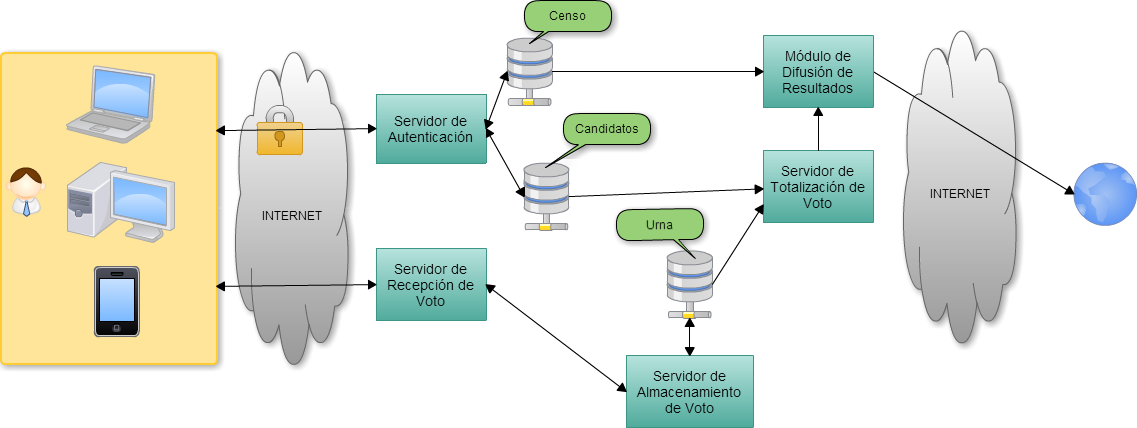
\includegraphics[width=1\textwidth]{imgs/sistema.png}
		%\caption{Diagrama de flujo del Sistema}
		%\label{fig:sistema}
	%\end{figure}
	%
	%\begin{figure}[htbp]
		%\centering
			%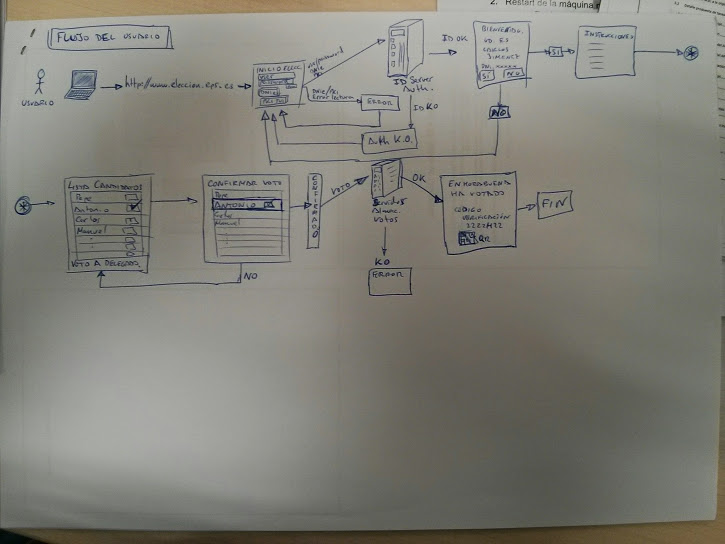
\includegraphics[width=0.60\textwidth]{imgs/flujoUsuario.jpg}
		%\caption{Esquema del flujo que sigue el votante}
		%\label{fig:flujoUsuario}
	%\end{figure}
	%\begin{figure}[htbp]
		%\centering
			%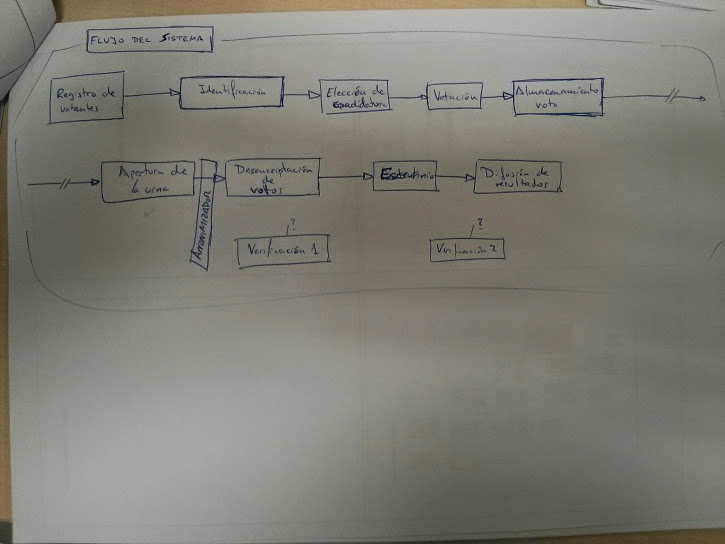
\includegraphics[width=0.60\textwidth]{imgs/flujoSistema.jpg}
		%\caption{Esquema del flujo del Sistema}
		%\label{fig:flujoSistema}
	%\end{figure}
	
		
		\section{Dise�o}\label{dise�o}
			\subsection{Dise�o del esquema de votaci�n}\label{disenhoEsquemaVoto}
				\subsubsection{Registro}
					La fase de registro de votantes en el sistema no ser� interactivo en cuanto a que no es el propio votante el que debe inscribirse para poder votar en las elecciones, sino que es la Autoridad Electoral la que lo registra en el censo. En esta fase, pues, se trata de establecer el censo de votantes que tienen autoridad para votar en el proceso electoral.
					
					Como se advierte en el an�lisis se ha tomado en consideraci�n que sean los administradores del sistema quienes tengan responsabilidad sobre el tratamiento del censo, por lo que se ha de cargar en el sistema y �ste es el que lo va a tratar.
					
					El censo ha de cargarse en dos servicios del sistema, tanto en el servidor de autenticaci�n como en el sistema de votaci�n.
					
					El censo del subsistema de autenticaci�n se utilizar� para llevar el control de los votantes que tienen derecho de acceso al sistema, por lo que a los votantes se les puede a�adir otros usuarios necesarios para llevar a t�rmino la votaci�n, como pueden ser administradores o auditores, aunque estos no tengan derecho de voto. As� se conformar�a la base de usuarios activos del sistema.
					
					En el subsistema de voto tambi�n se vuelca el censo para cada uno de los diferentes procesos de voto que conformen la elecci�n.
					
					El procedimiento a seguir consistir� en que la Autoridad Organizadora del Proceso Electoral, la Universidad, proveer� una lista del censo a los administradores del sistema. El administrador utilizar� la funci�n de carga de votantes con la lista proporcionada para realizar la carga inicial de votantes para cada una de las subelecciones que se configuren.
					
					La lista proporcionada por la Universidad debe contener la siguiente informaci�n de cada uno de los votantes:
						\begin{itemize}
							\item Nombre y apellidos
							\item DNI
							\item Clase / grupo de votantes
							\item E-mail
						\end{itemize}
						
					La carga de los votantes a trav�s de su aplicaci�n se realiza subiendo un fichero csv con la informaci�n requerida. Este fichero se pone a disposici�n de la cola de procesos, la cual, llegado el momento volcar� cada uno de los registros en la base de datos del sistema de votaci�n.
					
					\notasDuda{Falta definir el proceso de carga de votantes para el servicio de autenticaci�n.}
					
				\subsubsection{Identificaci�n}
					El servicio de identificaci�n es un subsistema clave en el proceso electoral. En �l recae parte de la responsabilidad de la robustez del sistema, en cuanto a que debe asegurar varios de los requisitos b�sicos que definen el voto electr�nico en concreto:
					
		\notasInfo{Esto es as� seg�n los requisitos de Fujioka, si se utilizan los de la UNEX, se puede modificar.}
		\begin{description}
			\item[Solidez:] Debe asegurar que un votante deshonesto no tenga capacidad de acceder al sistema e interrumpir la votaci�n. Es decir, que s�lo debe dar acceso a los votantes que realmente deben ingresar al sistema de votaci�n.
			
			\item[Elegibilidad:] Este requisito implica que el sistema debe controlar que ning�n votante que no tenga permitido el voto pueda votar. Aunque es el proceso de votaci�n el que debe controlar esta circunstancia cuando un usuario trata de emitir un voto, el sistema de votaci�n, de forma an�loga al requisito anterior, tambi�n debe proteger el sistema evitando el acceso a aquellos que, directamente, no tengan permisos para votar.
			
			\item[Sin duplicados:] El sistema debe evitar que un votante duplique o reemplace el voto de otro. Igualmente, aunque es el sistema de votaci�n el que debe tener mecanismos que controlen esta situaci�n, la primera barrera debe ser la servicio de autenticaci�n del votante.
			
		\end{description}

					
			 El sistema de identificaci�n del votante se apoya en el protocolo oAuth2.				
					
					
					
					
					
					
					
					
					
					
					
				\subsubsection{Elecci�n de candidatura}
				\subsubsection{Votaci�n}
				\subsubsection{Escrutinio}
				\subsubsection{Difusi�n de resultados}
				
			\subsection{Dise�o de la arquitectura}
			\subsection{Dise�o de la capa de datos}
			\subsection{Dise�o de la red}
			\subsection{Dise�o de la interfaz de usuario}\label{dise�o_interfaz_usuario}
				\subsubsection{Estructura de la p�gina web}
				\subsubsection{Estructura de la aplicaci�n m�vil}
				\subsubsection{Colores}
				\subsubsection{Logo de la elecci�n}
			
				\subsubsection{Ergonom�a}
				
				
				
				\todo[inline]{Desde aqu� hasta el comienzo de \ref{solucion_protocolo} hay que moverlo a An�lisis.}
				En varios de los sistemas estudiados que se han desarrollado para intentar implantar el voto electr�nico a un nivel medio, como pueden ser los mexicanos SELES \ref{seles} y SEVI \ref{sevi} o los espa�oles de V�ctor Moreno \cite{moreno07} \notasDuda{???????}o Votescript \ref{ivotingVotescript}\notasDuda{???????} se observa que se realiza una divisi�n del proceso electoral en cuatro fases (Registro, Votaci�n, Consolidaci�n de resultados y Auditor�a). En el desarrollo de este sistema vamos a identificar las mismas fases, pero con matices.
				
				As�, en una primera visi�n global del sistema, en este se definen cuatro fases:
				\begin{itemize}
					\item Preelectoral
					\item Votaci�n
					\item Consolidaci�n de resultados
					\item Postelectoral
				\end{itemize}
				
				Realmente, la mayor diferencia con las fases definidas en los esquemas anteriores se corresponden con el alcance de la primera y la �ltima fase.
				La fase Preelectoral, denominada com�nmente en los ejemplos estudiados en la Introducci�n como fase de Registro, en este sistema tiene un alcance mayor. En este proceso electoral no se requiere que el votante se registre para poder votar. El censo lo proporciona la Autoridad Electoral y se carga en el sistema. Igualmente, en los d�as previos a la jornada electoral el sistema permitir� a los votantes comprobar si est�n en el censo y qu� informaci�n contiene �ste, tanto personal - para asegurarse de que podr�n identificarse - como de permisos de cara a realizar la votaci�n.
				
				La fase postelectoral, que denominan de Auditor�a, preferimos dejarla como postelectoral al considerar que la auditor�a del sistema es una operativa que se realiza durante toda la jornada electoral, no s�lo al finalizar �sta. No obstante, es cierto que al final se llevar�n a cabo auditor�as de los resultados y el funcionamiento. Adem�s de las auditor�as llevadas a cabo por los auditores \textit{oficiales}, se va a implementar un mecanismo que permita a los propios votante auditar que su voto ha sido correctamente incluido y contado en el proceso. Esta fase postelectoral tambi�n tiene m�s operativas ... \todo[inline]{continuar con fase postelectoral}
				
				Las fase de votaci�n tambi�n tiene un alcance diferente. En primer lugar, empieza con la identificaci�n del votante en el sistema electoral. Una vez el votante ha sido correctamente identificado por el sistema (tal como lo har�a contra los miembros de la mesa en el voto tradicional), debe recibir una boleta electr�nica que le ofrezca las opciones entre las que, por su circunscripci�n, deba elegir la que desea votar. Una vez seleccionado, es el momento en el que realmente el votante realiza la votaci�n, traspasando el voto de forma digital al sistema, a la \textit{urna digital} donde se anonimizar�n y almacenar�n hasta la fase de consolidaci�n.
				
				En la fase de consolidaci�n de resultados, el sistema se encargar� del conteo de los votos que han sido emitidos
				\todo[inline]{continuar...}
				
			\todo[inline]{Antes de este punto hay que hacer un resumen de los diferentes esquemas de votaci�n, teniendo estos como Firma ciega, mixnets, etc...}

			\subsection{Protocolo}\label{solucion_protocolo}
			\textst{
				Como se ha comentado en cap�tulos anteriores, hay una multitud de soluciones propuestas para el voto telem�tico.
				
				Teniendo en cuenta el objetivo de este Proyecto Fin de Carrera, de los sistemas implementados a gran escala, a nivel nacional o regional, podemos destacar Estonia, Noruega y los cantones suizos como las tres experiencias m�s exitosas y aquellas de las que se pueden estudiar las soluciones, esquemas y protocolos utilizados. No obstante, el alcance de las mismas supera sobremanera el de este proyecto. Igualmente, muchas decisiones las toman en base a satisfacer requisitos que resultan muy importantes en su an�lisis, pero que en este trabajo no se ha considerado que tengan igual trascendencia, y viceversa, por lo que se han de tomar diferentes consideraciones frente a los mismos problemas dependiendo del impacto que suponen en cada proyecto.
				}
				Tambi�n se han presentado casos de proyectos de voto telem�tico pensados a menor escala. Entre ellos, hay muchas soluciones que, en parte, podr�an satisfacer los requisitos de este proyecto. No obstante en ninguno de ellos encontramos un protocolo que se adapte completamente a los requerimientos planteados, ya que, en alg�n momento, se analiza un elemento que los hace diferir. Por ejemplo, un proyecto ya maduro como Votescript (\ref{ivotingVotescript}) realiza un estudio acad�mico y t�cnico muy profundo acerca del voto telem�tico pero, por su propia definici�n, el modelo de identificaci�n y emisi�n del voto lo sit�an f�sicamente en centros de votaci�n. Este elemento es diferencial para este proyecto, pensado en el voto telem�tico remoto, aunque puede integrarse cuando se estudian alternativas para que aquellos votantes que, por alg�n motivo, no pueden o quieren votar por Internet de forma remota tengan la oportunidad de ejercer su derecho de sufragio desde un lugar habilitado para ello por la propia Escuela.
				\textst{
				A partir de los esquemas criptogr�ficos estudiados y con ayuda de algunos protocolos ya publicados en otros proyectos, el siguiente paso es dise�ar el protocolo de votaci�n que se adapte a las necesidades del Proyecto, cumpliendo con los requisitos y asegurando los niveles de seguridad planteados.
				
				En muchas de las soluciones estudiadas se observa que no recibe la importancia necesaria la fase de identificaci�n del votante. Los mecanismos de identificaci�n y autenticaci�n del mismo resultan laxos desde el punto de vista de la seguridad ante el fraude electoral. Por ello han sido descartadas las soluciones basadas en identificaci�n por medio de bases de datos con el t�pico protocolo de usuario/contrase�a o incluso con elementos de seguridad de una generaci�n algo posterior, como pin, patrones, captchas, operaciones aritm�ticas o m�todos similares con mayor o menor complejidad. Igualmente, se han descartado aquellos m�todos de identificaci�n que requieran la presencia f�sica del votante frente a los responsables de la mesa de votaci�n, ya que se busca el dise�o de un sistema remoto. As� descartamos protocolos de identificaci�n como los publicados por Votescript, en el que el votante acude a un centro o local de votaci�n, se identifica ante la mesa electoral y recibe un token criptogr�fico personalizado con el que se le permite ejercer el sufragio.
				
				La mayor�a de las soluciones estudiadas previamente a la realizaci�n de esta memoria centran sus esfuerzos en la fase de votaci�n. Buscan la elaboraci�n de un protocolo robusto, basado en esquemas criptogr�ficos, que permita la mayor seguridad posible al cumplimiento de los requisitos fundamentales del voto electr�nico, dotando al sistema de privacidad del votante, 
			}
				\todo[inline]{Hay que modificarlo. Es anterior a la decisi�n de utilizar Helios}
				
				
				
				
				
				
				
				
				
				
				
				
				
				
				%\subsubsection{Descripci�n del sistema}\label{solucion_descripcion}
				%El sistema contar� de cinco fases, determinadas por el flujo temporal de la votaci�n.
				%Preelectoral, Identificaci�n, Votaci�n, Escrutinio y publicaci�n de resultados.
				%Adicionalmente, se tendr� en cuenta un sistema de auditor�a, de car�cter transversal a este flujo, ya que debe estar disponible durante todo el proceso de votaci�n.
				%
				%\todo[inline]{No he podido conseguir reglamentaci�n oficial de la elecci�n, as� que, b�sicamente, propongo yo las fases y la problem�tica ... esto, con palabras aqu� escrito y bien puesto }
				%
				
				
				\section{ESTO ES EL PFC}
				\todo[inline]{ESTO NO VA EN EL PFC, ES UNA EXPLICACI�N PARA TENER PRESENTE QU� ES EL PFC YU PODER DESARROLLAR LA MEMORIA EN TORNO A LA IDEA QUE TENEMOS.}
				El sistema que se propone en este PFC es un sistema integral. Busca sostener el proceso electoral desde el comienzo hasta el final del mismo. Por ello empieza en el momento mismo de definici�n del censo y no termina hasta que la publicaci�n de resultados y su auditor�a son oficializadas por el �rgano rector de la Elecci�n.
				
				La primera fase, preelectoral, es aquella previa al d�a electoral, en la cual se definen las bases en las que se rige el proceso electoral.
				
				As�, es imprescindible cumplimentar varias acciones por parte de los desarrolladores, administradores y �rgano electoral.
				
				En primer lugar, es fundamental la elaboraci�n de un censo electoral. En �ste se recogen los potenciales votantes, aquellos con derecho a voto, identificando, adem�s, la circunscripci�n \notasDuda{Cir-cuns-crip-ci�n??? No hay una forma mejor de expresarlo??} a la que pertenece. En unas elecciones legislativas, una circunscripci�n electoral se puede definir como el conjunto de electores a partir del cual se procede la distribuci�n de los esca�os asignados, en funci�n de la distribuci�n del los votos sufragados. En las elecciones legislativas espa�olas, las circunscripciones se corresponden con las provincias espa�olas (excepto en el caso de Aturias, que est� subdividida en 3 distritos electorales, y la Regi�n de Murcia, que lo hace en 5). Esto significa que del total de diputados que se eligen en este proceso para la totalidad de Espa�a, en vez de repartirlos con el recuento total de los votos, se reparten los cargos por cada circunscripci�n, dependiendo del n�mero de electores de cada una, con lo que los votantes censados en una circunscripci�n, digamos por ejemplo la provincia de M�laga, elegir�n a un n�mero determinado de diputados que ser�n quienes les representen en el Congreso junto a los elegidos en el resto de territorios espa�oles. En las Elecciones al Parlamento Europeo, sin embargo, Espa�a act�a como una �nica circunscripci�n, por lo que los diputados que representar�n al pa�s en la c�mara supranacional se obtendr�n a base de repartir los esca�os con respecto al total de votos recogidos en todo el territorio espa�ol.
				
				Algo parecido es lo que se va a definir en el censo electoral. Adem�s de recoger de forma un�voca a los electores con derecho al voto, se tendr�n que sumar las ************\notasCambio{*********} necesarias para su correcta identificaci�n, as� como la ``circunscripci�n'' a la que pertenece, es decir, el grupo sobre el que debe escoger a sus representantes, con el fin de que la opci�n de voto que el sistema le presente y la que introduzca en el sistema sea correcta.
				
				Se vislumbran aqu� dos requisitos del voto electr�nico que necesitan ser satisfechos para la integridad del proceso electoral.
				
				En primer lugar, es b�sico que el censo defina claramente los votantes con derecho al voto y provea de la informaci�n necesaria para que se pueda comprobar la identidad del votante en el momento en el que se disponga a votar. En las elecciones con voto tradicional esto se consegu�a a�adiendo datos personales tales como el n�mero del DNI, del Pasaporte o, en caso de estas elecciones, el n�mero de identificaci�n del alumno. As�, al acudir a la mesa electoral todos los votantes ten�an estos datos con los que se pod�an identificar frente a los miembros de la misma, los cuales tienen la potestad de permitirles votar o no.
				
				Integridad del voto. El hecho de relacionar cada votante con una ``circunscripci�n'' es esencial a la hora de mantener la integridad de la votaci�n, pues hay que tener en cuenta los candidatos a los que cada votante puede votar, ya que no son los mismos para todos. Igual que en unas legislativas espa�olas un votante de M�laga no elige entre los mismos candidatos que lo hace un votante de Lugo, en estas elecciones, un alumno elige sus representantes entre los delegados de curso, mientras que los profesores, por su parte, lo hacen entre otros colegas profesores. Es indispensable, pues, gestionar correctamente estas relaciones ya que no se deben recoger votos de votantes a candidatos a los que no tiene derecho a elegir.
				
				En el caso de esta elecci�n, es la propia Escuela Polit�cnica Superior la que debe proveer el censo oficial a los administradores del sistema, los cuales proceder�n a cargarlo en el mismo a trav�s de los mecanismos implementados para ello.
				\notasInfo[inline]{(Aqu� encontramos un primer punto de auditor�a importante).}
				\notasInfo[inline]{(En algunos pa�ses, en vez de elaborarse un censo oficial, son los propios votantes los que han de registrarse)}
				
				
				Es requisito de la Instituci�n que convoca el proceso electoral el definir las ``reglas del juego''. En este caso, el �rgano de la EPS encargado de la celebraci�n de las elecciones ha de definir los mecanismos de votaci�n para que el sistema se pueda adaptar y mantener .......
				\todo[inline]{continuar...}
				
				Candidatos. Es necesario que los candidatos puedan presentar su candidatura e incorporarse al sistema para que �ste pueda gestionarlos para presentarlos como opciones a los votantes determinados, adem�s de en el momento de consolidaci�n de los votos y posterior publicaci�n de resultados.
				En muchos procesos se realizan desarrollos que permiten a los partidos pol�ticos registrar sus listas electorales y/o candidatos de forma remota durante el plazo determinado que la Ley Electoral les indica. As�, los partidos inscriben a sus representantes en el proceso electoral. En el caso de esta elecci�n, debido a su car�cter tan localizado no vemos necesidad de ello y corresponde a la Escuela Polit�cnica Superior proporcionar el listado de candidatos elegible y las circunscripciones a las que se presentan.
				\todo[inline]{Para futuros desarrollos, pensando en la escalabilidad del sistema, se podr�a desarrollar este punto para que este proceso sea independiente de los �rganos electorales de la EPS}.
				
				En las elecciones tradicionales, es tambi�n necesaria la formaci�n de las mesas electorales, con la definici�n del n�mero de ellas que son necesarias y la designaci�n de los miembros que van a formar parte de ella. En una elecci�n electr�nica y remota, como la que hemos dise�ado, el concepto de mesa se puede mantener, sobre todo para poder gestionar las circunscripciones y para continuar con las estad�sticas de participaci�n tradicionales, basadas en agrupaciones y disgregaciones de mesas. Sin embargo, al transformarse en un concepto l�gico, se pierde el sentido de la designaci�n de los miembros de mesa, por lo que no ser� un punto a tener en cuenta en el proceso.
				
				
				\todo[inline]{Pasamos a la siguiente fase: Identificaci�n}
				Una vez acometidas todas las gestiones de la fase preelectoral, pasamos a la fase correspondiente al llamado D�a Electoral (aunque realmente la elecci�n en vez de en un d�a, se pueda alargar a lo largo de un per�odo de tiempo mayor).
				Tratando de emular a las elecciones tradicionales, esta fase comienza con la apertura de los colegios electorales y las mesas que los componen. En el caso digital, ser�n los miembros designados por la Junta Electoral los que, previa identificaci�n y requerimiento de sus credenciales digitales, pongan en marcha el sistema en su fase electoral. Ser� una apertura de los colegios de forma virtual, permitiendo que los votantes puedan acceder al sistema y proceder a votar.
				La fase de identificaci�n del votante es una fase realmente importante. En las elecciones de voto tradicional, el proceso normal consiste en que el votante acude a la mesa electoral y muestra a los miembros de mesa alguna identificaci�n de curso legal, respaldada por alguna instituci�n estatal reconocida y capacitada. Los miembros de la mesa electoral contrastan la identificaci�n presentada con la informaci�n recogida en el censo electoral de dicha mesa y deciden si es suficiente o no para permitir al votante introducir su voto en la urna. En el caso de las elecciones legislativas espa�olas los documentos que se pueden mostrar son DNI, pasaporte o permiso de conducir. Todos estos documentos son v�lidos para votar incluso estando caducados. Han de mostrar la fotograf�a del votante para permitir la identificaci�n por parte de los miembros de mesa, por lo que, aunque sea v�lido que est�n caducados, no se permite utilizar el resguardo de DNI en tr�mite.
				\todo[inline]{En el caso de las elecciones de la EPS, los documentos v�lidos son .-......}
				Es requisito el sustituir este sistema de identificaci�n del elector por otro en el que no sea necesaria la presencia f�sica de �ste ni de los miembros de mesa para permitir el voto, aunque manteniendo el mismo nivel de seguridad en el proceso. Aqu� se hace indispensable estudiar las opciones de identificaci�n digital que se pueden implementar para .............
				\todo[inline]{continuar}
				
				Lo ideal es disponer de documentos que contengan tokens criptogr�ficos propios que puedan ser utilizados en los diferentes procesos de identificaci�n y voto. Por ello, vamos a utilizar documentos que los disponen.
				
				As�, los documentos v�lidos para ejercer el derecho al voto ser�n el DNIe (tanto la primera versi�n como la denominada 3.0, presentada en enero de 2015) y la TUI \notasMejorar{***InfoTUI***} de la Universidad San Pablo-CEU. En sendos documentos encontramos elementos criptogr�ficos que identifican un�vocamente a su due�o. Adem�s encontramos en ellos certificados para la firma digital, que ser�n necesarios para la fase de votaci�n.
				
				El votante se identifica con su documento digital de forma remota. Es necesario que disponga de un lector de chip electr�nico conectado al dispositivo desde el que va a realizar el voto, aunque utilizando DNIe con lector de chip sin contacto, no har�a falta si se hace uso de un dispositivo con sensor de radiofrecuencia, con capacidad para leer informaci�n a trav�s de NFC.
				
				A trav�s de la app Android (o la app web), el votante accede al servicio de votaci�n por Internet. El primer paso es la identificaci�n del votante. Es la primera vez que har� uso de los certificados del DNIe. En este caso, la app leer� (con NFC o chip con contacto) el certificado de Autenticaci�n del DNIe, por el cual se asegura la identidad del votante. Con la identidad del votante verificada (por la DGP), se contrasta con el censo, para comprobar:
				\begin{itemize}
					\item Si el votante existe en el censo.
					\item Si el votante ha votado previamente.
					\item Los datos censales del votante, para comprobar circunscripci�n, mesa electoral y, por ende, ser capaz de obtener los candidatos entre los que puede escoger.
				\end{itemize}
				
				Una vez verificado el votante y comprobados sus datos censales, se procede a construir la boleta con los candidatos que entre los que le corresponde elegir bas�ndose en su circunscripci�n electoral. El sistema ha de presentar la boleta al votante y permitir que �ste marque la o las opciones que permita el sistema electoral para constituir el voto a emitir.
				
				Una vez constituido el voto (papeleta), hay que proceder a la votaci�n digital. Para ello nos basamos en cifrado y firma ciega. As�, el primer paso es que la app utiliza la clave p�blica de la Entidad Electoral para cifrar el voto. Con el voto cifrado, el votante ha de firmarlo. La firma se realiza con el certificado de Firma que posee el DNIe. As�, el votante firma un conjunto de [voto cifrado + votante], que es el paquete que se pasar� al subsistema de gesti�n del voto.
				
				Una vez el votante ha emitido el voto, el sistema le devuelve un resguardo (c�digo QR como en Estonia, un c�digo alfanum�rico, no s� todav�a) con el cual puede verificar que el voto ha sido correctamente incluido en el sistema. Adem�s, podr� verificar que el voto ha sido correctamente incluido en el escrutinio. \notasCambio[inline]{(No s� si con este resguardo debe poder llegar a la opci�n de voto elegida, todo depende de c�mo tomemos el requisito de coerci�n y qu� es lo que menos le afecta)}
				
				El votante puede votar tantas veces como desee cambiar su voto \notasInfo{As� disminuimos el riesgo de coerci�n}. Para ello, hay un protocolo por el cual cuando un votante emite su voto, todos los anteriores son anulados. \todo[inline]{Hay que definir el protocolo para la anulaci�n de votos por 'revoto'}
				
				El sistema de gesti�n del voto es el encargado de los votos sufragados durante la jornada electoral. El sistema almacena los votos firmados (voto cifrado + votante) en una \textit{urna} digital durante el tiempo que dura la jornada electoral. En caso de recibir un voto de un votante que ya previamente hab�a emitido su voto, debe ser capaz de anular los votos anteriores que �ste hubiese sufragado\notasInfo{Como digo antes, hay que definir c�mo se hace esto de anular votos emitidos}.
				Una vez que el Administrador del Proceso Electoral da por terminada la Jornada Electoral, los Miembros de la Junta Electoral utilizan sus claves para formar la clave maestra que permite dar por terminada la fase de votaci�n y comenzar con el Escrutinio.
				La primera fase del Escrutinio es que los votos firmados deben ser \textit{anonimizados}. Esto lo vamos a realizar en dos pasos. Primero, comprobamos la validez de la firma del voto firmado. Si la firma se corresponde con u voto a descartar, se elimina. Si la firma es v�lida, se extrae (abrimos el sobre donde va la info del votante y el sobre con su voto secreto) del contenido del voto firmado tanto el voto cifrado como la informaci�n asociada del votante. Por un lado, la informaci�n del votante se almacena para sacar un listado de votantes (que podr� compararse con el resultado de votantes del censo). Por otra parte, los votos cifrados pasan a otro almac�n ya sin asociaci�n con su votante. Para terminar de separar los votos de sus votantes, pasamos por un proceso anonimizador que ... \todo[inline]{Aqu� entra en juego ElGamal y sus amigos o las mixnets}.
				Una vez tenemos los votos separados de sus votantes, procedemos a la siguiente fase del escrutinio, que es la de (abrir el sobre del voto secreto) descifrar el voto. El sistema necesita la clave privada de la Entidad Electoral para descifrar los votos que, recordemos, est�n cifrados con la clave p�blica. Con esta clave privada, extraemos el contenido del voto cifrado y obtenemos cada uno de los votos en plano de las urnas digitales.
				Una vez obtenidos el conjunto de los votos en plano de cada urna digital, podemos proceder a la consolidaci�n de los votos. Se realiza el conteo de cada urna y, con los resultados obtenidos, se puede realizar la totalizaci�n para llegar al resultado final de la Elecci�n.
				
				El �ltimo paso del sistema ser� el de la Difusi�n de los Resultados. El sistema de Escrutinio (o Totalizaci�n) informa de los resultados al m�dulo de Difusi�n, el cual les aplicar� el formato necesario para cumplir con las necesidades de publicaci�n de los mismos. En el caso del Proceso Electoral asociado a este proyecto, una web y diversos listados PDFs para poder ser cotejados.

				Ser�a muy interesante que, como en Estonia, los votantes tuvieran una herramienta para poder verificar que su voto ha sido correctamente incluido y escrutado en el Proceso.
				
				Paralelamente a todo el proceso, cada subsistema ha de generar una serie de registros, ficheros logs, que puedan ser visualizados por un conjunto de auditores, observadores u otro grupo de profesionales que tengan que dar cuenta del correcto funcionamiento del Proceso y de la transparencia del mismo, as� como del �xito t�cnico del Sistema.
				
				
%%\chapter{Manuales}\label{manuales}
\lhead{Cap�tulo \ref{manuales}}
\rhead{Manuales}
%*******************************************************************************
\section{Notas sobre los manuales}
\par
El objetivo de este cap�tulo es facilitar unos manuales m�nimos pero suficiente para poder instalar, configurar, utilizar y administrar el sistema, de una forma correcta pero sencilla. 
\par
Aunque podr�amos entender que los contenidos de este cap�tulo podr�an estar dentro de los apartados relativos a la construcci�n del sistema y a la implantaci�n y despliegue, se ha optado por presentarlo a parte, debido a la importancia que tiene dentro de los requisitos descritos. Dicha importancia viene descrita en el apartado \ref{alcance_final}, sobre el alcance final del proyecto, donde se indicaba la creaci�n de los manuales como el tercero de los cuatro objetivos a resolver (los dos primeros quedaron resueltos en el cap�tulo \ref{solucion}, y el cuarto se resolver� en el cap�tulo \ref{lineas_futuras}).
\par
Si se precisa ayuda, o ampliar informaci�n sobre el sistem Linux, en quien reside la aplicaci�n, ver \cite{autounix}. Puede ser muy util tanto a la hora de la instalaci�n, configuraci�n, uso, administraci�n y mantenimiento del sistema.
\section{Manual de Instalaci�n}
\subsection{Requisitos para la instalacion}\label{requisitosinst}
\subsection{Pasos previos a la instalaci�n}
\par
Para poder realizar la instalaci�n de los programas necesitaremos previamente instalar la distribuci�n correspondiente de Linux, en este caso la distribuci�n SUSE 9.3, incluyendo los siguientes paquetes:
\begin{itemize}
\item
	python: int�rprete de Python (versi�n superior a TODO:qu� versi�n?)
\item
 	python-devel: paquete necesario, pues roundup necesita "distutils". Este paquete requiere de la instalaci�n de python-tk y blt.
\end{itemize}

\subsection{Instalaci�n de Roundup Issue Tracker}
\par
A continuaci�n se muestran las distintas acciones a seguir para una correcta instalaci�n y configuraci�n del programa.
	{Operaciones a realizar en modo superusuario}
\par
A continuaci�n se muestran los pasos a seguir, que deber�n ser realizados desde la consola, habi�ndose identificado como "root":

\begin{itemize}
\item
	Elecci�n de la direcci�n para la instalaci�n (en este caso, elegiremos: 
\begin{center}
\verb|/opt/roundup/bin| 
\end{center}
\item
	Ejecutar, situ�ndonos en el directorio donde hayamos descomprimido el programa:
\begin{center}
\verb|python setup.py install --install-scripts=/opt/roundup/bin| .
\end{center}
\end{itemize}
\par
Para cualquier duda que pueda surgir sobre la instalaci�n de roundup, se recomienda encarecidamente ver \cite{roundupweb}.
\par

\subsection{Instalaci�n PostgreSQL}\label{instpost}
\par
\textbf{DECIR LAS INDICACIONES PROPIAS QUE REQUIERE POSTGRES}
\par
Para cualquier duda que pueda surgir sobre la instalaci�n de roundup, se recomienda encarecidamente ver \cite{postweb} y \cite{postgres}.
\par
\subsection{Instalaci�n Xapian}\label{xapinst}
\textbf{DECIR LAS INDICACIONES PROPIAS QUE REQUIERE ROUNDUP PARA ESTO}
\par
Cualquier aclaraci�n adicional que se necesite sobre c�mo debe hacerse la instalaci�n de Xapian, se puede obtener en \cite{xapianweb}.
\par


\section{Manual de Configuraci�n}

\par
En este apartado trataremos sobre c�mo configurar e inicializar el tracker, as� como los complementos necesarios para el funcionamiento del sistema\footnote{Tenemos que tener en cuenta que, como ya hemos comentado en el apartado \ref{decisiones}, utilizaremos el usuario ''\textbf{pfc}''.}.

\subsection{Configuraci�n de los elementos complementarios}
\subsubsection{Configuraci�n de la base de datos}

\subsection{Configuraci�n del tracker}
Para configurar el tracker, se deber�n seguir los siguientes pasos (todos ellos en modo superusuario):
\begin{enumerate}
	\item Crear directorio para incluir el tracker \footnote{NOTA: en el caso hipot�tico de que futuras verisiones consideraran que deber� configurarse m�s de un tracker, se utilizar� un �nico directorio para todos.}. 
\begin{center}
\verb|mkdir /opt/roundup/trackers|
\end{center}
	\item A�adir al path la direcci�n donde se encuentran los scripts (en nuestro caso en /opt/roundup/bin
	\item Ejecutar el siguiente comando: \verb|roundup-admin install|. Al ejecutarse esta opci�n, la aplicaci�n nos pedir� que seleccionemos la plantilla (template) y el sistema gestor de bases de datos subyacente (backend) a utilizar:
\begin {itemize}
	\item Inserte directorio base (Enter tracker home): en nuestro caso introduciremos:
\begin{center}
\verb|/opt/roundup/trackers/pfc/|.
\end{center}
	\item Seleccione plantilla (Select template):por defecto introduciremos 'classic'.
	\item Seleccione base de datos (Select backend): por defecto introduciremos 'anydbm'.
\end {itemize}
	\item Realizaremos las siguientes modificaciones en el archivo 'config.ini'\footnote{NOTA: para facilitar la configuraci�n, se adjunta en el cd de instalaci�n una versi�n del fichero config.ini que podr� tomarse tal cual para sustituir la que genera por defecto.}, cuyo sentido se explica en el apartado \ref{config}, sobre el dise�o de la aplicaci�n. (para lo cual, comprobaremos los correspondientes permisos y ajustaremos seg�n sea preciso):
\begin {itemize}
	\item \verb|[main]|
\begin {itemize}
	\item \verb|admin_email = pfc|
	\item \verb|dispatcher_email = pfc|
\end {itemize}
	\item \verb|[tracker]|
\begin {itemize}
	\item \verb|web = http://localhost:8080/pfc|\footnote{NOTA: Esta direcci�n deber� ser modificada de acuerdo a la ubicaci�n que tenga el equipo que sirva realmente la aplicaci�n. Indicar Localhost �nicamente valdr� para un escenario de pruebas en que cliente y servidor est�n en el mismo equipo}
	\item \verb|email = pfc|
\end {itemize}
	\item \verb|[mail]|
\begin {itemize}
	\item \verb|domain = localhost|
	\item \verb|host = localhost|
\end {itemize}
	
\end {itemize}
\end {enumerate}
\par
Para cualquier duda que pueda surgir sobre sobre la configuraci�n de roundup, se recomienda encarecidamente ver \cite{roundupweb}.
\par
\subsection{Inicializaci�n del tracker}\label{inicializacion}
\par
Antes que nada, hay que tener en cuenta que se tienen que verificar los permisos antes y despu�s de realizar este paso, pues al crearse nuevas carpetas puede ser que los permisos de �stas nos impidan realizar alg�n paso.
\par
La inicializaci�n del tracker debe hacerse tambi�n como superusuario. Los pasos a seguir ser�n los siguientes
\begin{enumerate}
	\item Se ejecutar� el comando:
\begin{center}
\verb|roundup-admin initialize|
\end{center}
	\item Se nos pedir� introducir el directorio base del tracker:
\begin{center}
\verb|/opt/roundup/trackers/pfc/|
\end{center}
	\item Se nos pide introducir una contrase�a de administraci�n (en este caso hemos utilizado 'pfc')
\par
\end{enumerate}


\section{Manual de Uso}
\par
Una vez configurado el programa, e inicializado el tracker, en este cap�tulo se indicar� c�mo se debe proceder a levantar el servicio. Tambi�n se realiza alguna peque�a aclaraci�n sobre los distintos manuales que se deben utilizar.
\subsection{Levantar el servicio}\label{levantar}
\par
Para arrancar el tracker y que el sistema entre en funcionamiento, se debe levantar el servicio. 
\par
Esta operaci�n se deber� realizar tambi�n en caso de que la m�quina caiga, o tras cualquier operaci�n de mantenimiento del sistema. Es decir, cada vez que ocurra un evento por el cual debamos volver a poner en funcionamiento el sistema.
\par
Para levantar el servicio, deberemos trabajar como usuario normal, y no como superusuario (como hemos hecho en la instalaci�n y en la configuraci�n). Para ello, se deben revisar los permisos en las carpetas involucradas, y comprobar que sean los pertinentes.
\par
Se ejecutar�n en la consola las siguientes instrucciones, de acuerdo a los casos expuestos en la instalaci�n y la configuraci�n:
\begin{center}
\verb|export PATH=$PATH:/opt/roundup/bin|
\end{center}
\begin{center}
\verb|roundup-server pfc=/opt/roundup/trackers/pfc|
\end{center}
\par
Por comodidad en el uso, se recomienda encarecidamente el uso del script ''levantar.sh'' que se adjunta en el CD, y contiene s�mplemente esas dos instrucciones. Para utilizar este script, habr�a que alojarlo dentro del directorio ''home/pfc''. Para levantar la aplicaci�n bastar� unicamente con situarnos en ese directorio desde la consola y ejecutar:
\begin{center}
\verb|./levantar.sh|
\end{center}
\par
\subsection{Manual de usuario}
\par
Para un correcto uso del sistema, se ven involucrados los siguientes documentos:
\begin{itemize}
	\item Documentaci�n de uso de Round-up Issue Tracking (incluida en el CD adjunto, y tambi�n disponible y actualizada en \cite{roundupweb}).
	\item Cualquier manual, normativa o documentaci�n propuesta para la utilizaci�n de este sistema, comunicaci�n en los roles m�s bajos, etc, as� como cualquier otro documento que sea considerado pertinente por las Fuerzas Armadas.
\end{itemize}
\par
Aunque el funcionamiento del sistema es muy intuitivo y sencillo, cualquier duda podr� ser aclarada en la documentaci�n del programa, por lo que esa documentaci�n debe estar disponible. \par
Igualmente, el programa no deber� entrar en producci�n hasta que los usuarios finales tengan pleno conocimiento de las normativas de uso impuestas por las Fuerzas Armadas. 
 \label{uso}
\section{Notas sobre la administraci�n y el mantenimiento}
Hablar de que existe m�s documentaci�n para los backend,selenium etc.

Hacer una aclaraci�n sobre las cosas que debe hacer el administrador. (crear usuarios... ver guia de administraci�n de roundup
 \label{notasadmin}

%%\chapter{Lineas Futuras} \label{lineas_futuras}
\lhead{Cap�tulo \ref{lineas_futuras}}
\rhead{Lineas Futuras}
\section{Aclaraciones sobre las lineas futuras}
\par
En el apartado \ref{alcance_final}, sobre el alcance final, se defin�an cuatro objetivos a alcanzar en este proyecto. El primer objetivo y el segundo (encontrar un modelo y estructura v�lidos, y encontrar una soluci�n software v�lida) quedan resueltos en el cap�tulo \ref{solucion}. El tercer objetivo (Creaci�n de manuales) queda resuelto en el cap�tulo \ref{manuales}.
\par
El cuarto objetivo planteaba la necesidad de dar todas las facilidades posibles a futuras l�neas de desarrollo. A lo largo de todo el proyecto, cada vez que se ha tomado una decisi�n, se ha tenido en cuenta este objetivo. A lo largo de este cap�tulo se dar�n indicaciones adicionales y aclaraciones para cumplir finalmente este �ltimo objetivo.
\par
De entre todas las decisiones tomadas a lo largo del proyecto, hay que destacar el empleo del dise�o dirigido por pruebas, que facilitar� cualquier modificaci�n o ampliaci�n al sistema, aprovechando que las pruebas que deber�n superarse ya est�n programadas. Para mayor informaci�n sobre este punto, ver \cite{} y los apartados \ref{metod} y \ref{pruebas}.
\par
\section{Siguientes fases de desarrollo}
\par
En el apartado \ref{fases} se indicaba que este proyecto se correspond�a con la primera fase del desarrollo de un sistema de telemedicina militar mucho m�s amplio. La principal linea futura a seguir, despu�s de este proyecto, ser� la ejuci�n de las siguientes fases. Para satisfacer el �ltimo objetivo de este proyecto, ser� necesario facilitar ese futuro trabajo.
\par
A lo largo de todo el documento, se ha podido apreciar como las decisiones siempre se han tomado teniendo en cuenta estos futuros desarrollos. En todo momento se ha mostrado qu� decisiones se han tomado para la creaci�n de este primer prototipo, y las orientaciones convenientes para las siguientes fases de desarrollo, orient�ndonos ya en el despliegue del sistema real. Por este motivo, ser� fundamental la lectura del apartado \ref{solucion} para una buena consecuci�n.
\par
Adem�s de lo comentado en el apartado \ref{solucion}, a continuaci�n (y como ayuda a futuras mejoras que se quieran a�adir para implantarse en el sistema real) se describen algunas indicaciones importantes que se deber�n tener en consideraci�n para el desarrollo de dichas fases. No obstante se quiere recordar la importancia de la lectura de todo el apartado \ref{solucion}, y de la consulta a la bibliograf�a aportada, en los casos que sea preciso.
\par
\subsection{Modelo de despliegue real}
\par
El principal planteamiento que se deber� tomar en las futuras fases dentro del desarrollo es el modelo de despliegue que se deber� seguir. 
\par
Como se expone en este documento, los futuros desarrolladores no deber�an alejarse del modelo descrito en la figura \ref{fig:sistema_distribuido}, dentro del apartado \ref{modelo}, ya que dicho modelo encaja perfectamente con el sistema real expuesto en \ref{sistemareal}.
\par
En caso de decidirse emplear alg�n otro tipo de modelo de despliegue, tampoco deber�a ser complejo, pues la aplicaci�n a utilizar seguir� siendo la misma, y no se obligar�a a replantear ninguna otra caracter�stica ajena al propio despliegue.  
\par
\subsection{Soporte para el despliegue}\label{soport}
\par
Cuando se realice el despliegue en futuras fases, deber� plantearse cambiar las m�quinas sobre las que se instalar� la aplicaci�n. En este proyecto se propuso la instalaci�n sobre PC, pero cuando en fases posteriores sea desplegado todo el sistema, podr�a resultar interesante utilizar otro tipo de equipos.
\par
La f�cil adaptaci�n del sistema a un sistema operativo Solaris, podr�a dar como una buena opci�n utilizar m�quinas SUN. Pero en cualquier caso, al ser Unix un sistema multiplataforma en general, el principal argumento para cambiar los equipos donde instalarse ser� la propia decisi�n del cliente y de los administradores.
\par
\subsection{Cambio de Backend}
\par
El cambio de esta fase a las posteriores, donde ya nos adentraremos en el sistema real, y por tanto existir� un nivel de carga mucho mayor, requerir� plantearse la aplicaci�n de este cambio.
\par
En el apartado \ref{bd}, justificabamos que, si bien para este prototipo ser�a suficiente usar AnyDBM, en futuras fases la opci�n m�s razonable ser�a la utilizaci�n de PostgreSQL. 
\par 
Para la utilizaci�n de PostgreSQL se deber�n tener en cuenta varias cosas:
\par
\begin{itemize}
	\item En el momento de la instalaci�n del sistema, se deber�n tener en cuenta las indicaciones para instalaci�n de Postgres que se facilitan en el punto \ref{instpost}.
	\item En el momento de configuraci�n, deber� replantearse dentro del fichero config.ini el apartado [rbdms]. En el apartado \ref{config} se aporta una configuraci�n que deber�a ser v�lida, pero deber� reconsiderarse seg�n las opciones que se tomen a la hora de la isntalaci�n de PostgreSQL, as� como nuevas sugerencias o indicaciones de los administradores del sistema.
	\item Como su uso ralentizar� los accesos, se deber�a plantear la inclusi�n de Xapian en el sistema (ver apartado \ref{usoxap}).
	\item Se deber� estudiar la conveniencia de que la base de datos resida o no en la misma m�quina que Roundup, si bien hay que aclarar que en principio en este proyecto no se ha contemplado ning�n motivo que pueda empujar a tomar esta decisi�n.
\end{itemize}
\par
Para ampliar informaci�n sobre PostgreSQL, ver \cite{postgres} y {postweb}.
\par
\subsection{Uso de Xapian}\label{usoxap}
\par
El inconveniente que encontr�bamos en el uso de Roundup era una menor velocidad que si us�bamos otros SGBD, como se mostraba en la tabla \ref{tab:ComparativaSGBD}. En el apartado \ref{bd} se indicaba como algo interesante la utilizaci�n de Xapian para acelerar las b�squedas.
\par
Para la �ncorporaci�n de Xapian en el sistema, se debe consultar el apartado \ref{xapinst}, donde se aportan indicaciones sosbre la instalaci�n, y se puede ampliar informaci�n en \cite{xapianweb}.
\par

\subsection{Cambio de sistema operativo}
\par
En principio, si en fases posteriores se siguen instalando los servidores en PC's, no tiene ning�n sentido el cambio de sistema operativo, ya que Linux es totalmente v�lido. �nicamente podr�a plantearse el cambio de distribuci�n, pero siempre y cuando se trate de una distribuci�n fiable (ver apartado \ref{suse}).
\par
No obstante, en caso de optar por cambiar los servidores a m�quinas Sun, como se suger�a en el apartado \ref{soport}, se recomienda plantearse la utilizaci�n de Solaris.
\par
\subsection{Mejoras Interfaz}
\par
Otro aspecto que se deber�a plantear si se mejora en las siguientes fases es la interfaz. Seg�n los requisitos planteados, en principio ser�a suficiente con la interfaz web, como se describ�a en el apartado \ref{interfaz}. Pero en caso de considerarse cualquier tipo de mejora, podr�n realizarse las siguientes mejoras (para mayor informaci�n ver la documentaci�n actualizada disponible en \cite{roundupweb}.
\par
Otras opciones como aportar una interfaz email, o crear una interfaz a medida a partir de la salida por linea de comando que aporta Rondup, pueden ser planteadas seg�n nuevos requisitos que se puedan exigir en siguientes fases. 
\par
Finalmente, se podr�an requerir en futuras fases tambi�n cambios en la propia interfaz web ya presente, los cuales podr�an hacerse f�cilmente creando nuevas css, sin necesidad de cambiar nada m�s.
\par
\subsection{Sistemas de Backup}
\par
En fases futuras, habr� que prever sistemas de backup, para impedir que la informaci�n en cada servidor pueda perderse en caso de ocurrir alguna eventualidad o catastrofe.
\par
Ser� imprescindible desarrollar un sistema que guarde la informaci�n de los tickets de cada uno de los servidores ubicados en unidades de rol 2, en una unidad de rol 3 (o incluso 4, este aspecto deber� ser determinado, en base a las normativas ya existentes para comunicaci�n entre roles 3 y 4, y a las necesidades que las Fuerzas Armadas puedan requerir llegado el momento del despliegue).
\par
Puesto que la informaci�n es gestionada por un sistema gestor de bases de datos, la informaci�n en �ste contenida ser� lo susceptible a ser resguardado. Por tanto, los sistemas de backup a dise�ar, ser�n los de las propias bases de datos.
\par
Para mayor informaci�n sobre c�mo realizar el backup, as� como cualquier otra labor de administraci�n sobre la base de datos PostgreSQL ver \cite{postgres} y {postweb}.
\par
\subsection{Sistema de log}
\par
En este proyecto no se ha contemplado la necesidad de utilizaci�n de un sistema de logging. En las siguientes fases, si se considera apropiada su utilizaci�n, deber�n cambiarse los par�metros del fichero config.ini del apartado [logging], seg�n se indica en el apartado \ref{config}.
\par
\section{Otros �mbitos de aplicaci�n}
\par
Como futuras lineas de desarrollo de este proyecto, fuera del proyecto global al que pertenece, podr�an plantearse otros ambitos de aplicaci�n donde encajar�a tambi�n este sistema, en condiciones muy similares.
\par
\begin{itemize}
	\item \textbf{Telemedicina Civil.} El sistema es �ptimo para su utilizaci�n en medicina, no solamente militar, sino tambi�n civil. La adaptaci�n de este sistema a un sistema civil, �nicamente requerir�a de un replanteamiento del modelo de despliegue, pues el funcionamiento ser�a el mismo. No solo se podr�a utilizar a nivel de lo planteado este proyecto en concreto, el sistema de eventos, sino utilizarlo integrado al sistema de fichas m�dicas (que tambi�n deber�a adaptarse) tambi�n desarrollado en distintas fases.
	\item \textbf{Sistemas dirigidos por eventos.} En general, cualquier sistema cuyo cambio de estados sea dirigido por eventos podr� ser susceptible de ser solucionado con la implantaci�n de esta misma soluci�n. Podemos destacar, a modo de ejemplo:
	
\begin{itemize}
	\item Sistema de carta electr�nica de un restaurante. La petici�n de un men�, que el plato est� listo, que el plato se sirva, que se pida la cuenta, que se pague: son eventos que hacen cambiar el estado del pedido, que en este caso ser�a el ticket.
	\item Sistemas de atenci�n al cliente y atenci�n t�cnica. La incidencia ser� el ticket en este caso, y se registrar� cada vez que se asigne a un nuevo personaje, se a�adan comentarios, haya cambios en el estado de la incidencia, etc.
	\item Tratamiento de siniestros en compa�ias aseguradoras. El concepto ser�a el mismo que el anterior, siendo cada parte de siniestro el equivalente a un ticket.
	\item Sistemas de asignaci�n de actividades en un proceso empresarial. Una actividad que va pasando de mano en mano, puede ser asignada con facilidad con un sistema como este.
\end{itemize}
\par
Esto es solo un ejemplo de las utilidades que podr�an darse a este sistema, pero hay infinidad de casos donde su utilizaci�n es la soluci�n m�s apropiada.
\end{itemize}



%%\chapter{Conclusiones}\label{conclusiones}
\lhead{Cap�tulo \ref{conclusiones}}
\rhead{Conclusiones}

	El problema del voto por Internet es m�s complejo de lo que a priori puede parecer.
	
	El hecho de tener que lidiar con el reto de la dualidad verificsbilidad - secreto (\ref{estadocuestion.votoelectronico.verifvssecreto}) complica el dise�o de cualquier sistema de voto electr�nico por Internet. Es muy complicado llegar al punto medio en el cual la privacidad del voto de un votante se mantiene lo justo para poder demostrar que el voto es correcto y de la misma forma ha sido inclu�do en el escrutinio.
	
	Esta lucha entre verificabilidad y secreto provoca desconfianza. Tanto en los propios votantes, por la privacidad de su elecci�n. Como en los afectados por el resultado, que pueden dudar de la transparencia del sistema, de la honestidad del mismo a la hora de contar los votos sufragados.
	
	La mayor�a de los retos tecnol�gicos est�n superados. La seguridad de las comunicaciones, la identificaci�n digital de los votantes, las herramientas criptogr�ficas. Incluso en este proyecto avanzamos una prueba de concepto para utilizar el nuevo \gls{DNIe} 3.0 usando sensores \gls{NFC} para poder votar desde un dispositivo m�vil. A diario utilizamos sistemas que requieren una seguridad muy importante, como las transacciones bancarias, consultas m�dicas, \gls{VPN}s corporativas, etc. 
	
	Sin embargo, en la mayor�a de estos casos de uso, un fallo en estos sistemas es visible cuando ocurre, incluso demostrable. Si falla el sistema del banco y nos cobra irregularmente m�s dinero del que debe, lo podemos ver en el extracto de nuestra cuenta y reclamarlo, por ejemplo.
	
	En un sistema de voto por Internet, esto no es posible. Al menos si queremos asegurar la privacidad del votante. Si el sistema no totaliza correctamente nuestro voto, no tenemos forma de saberlo o demostrarlo si no procedemos a desencriptar e identificar, de alguna forma, nuestro voto en la "urna digital".
	
	La confianza es b�sica, por tanto, para estos sistemas.
	
	Otro problema importante es la coacci�n. La capacidad de que un sistema proteja al votante de presiones externas a la hora de emitir su voto.
	
	El desarrollo de este proyecto, basado en Helios Voting, es factible para llevar a cabo elecciones con bajo riesgo de coacci�n, como las de nivel universitario, organizacional o corporativas. En estos casos, aunque la importancia de la elecci�n puede variar, normalmente el riesgo de coacci�n al votante es bajo. No es lo mismo cuando hablamos de elecciones de cargos p�blicos, donde s� que se pueden producir presiones importantes al censo.
	
	Todav�a queda un largo recorrido para que el voto por Internet llegue a elecciones legislativas en Espa�a. Pese a que existe una lista de ejemplos de pa�ses o territorios en los que s� que se ha establecido esta tecnolog�a, siendo Estonia el m�ximo exponente, personalmente creo que en Espa�a no es posible hacerlo de corto a medio plazo.
	
	El primer escollo para implantar el voto por Internet en Espa�a se encuentra en la Constituci�n Espa�ola.

	
	
	Tecnol�gicamente es posible dise�ar e implementar sistemas de votaci�n remota seguros. Existen multitud de protocolos criptogr�ficos para asegurar el voto, conexiones seguras, formas de identificar digitalmente a los votantes. El problema no creo que sea la tecnolog�a. M�s bien, desde mi punto de vista, el problema principal es la confianza.
	
	
	En la Constituci�n Espa�ola, dentro de la Ley Electoral, se dispone un escenario para las elecciones tradicionales basado en la desconfianza de los partidos pol�ticos en el proceso. Por ello, hay multitud de testigos y conteo manual de los votos. Las mesas electorales constan de Presidente y dos vocales, con la posibilidad de estar acompa�ados de interventores de los diferentes partidos pol�ticos, designados para ser testigos del proceso de voto y conteo, controlando que no haya manipulaci�n del proceso.
	
	El de Espa�a es un sistema bastante seguro. Tiene riesgos de integridad y coacci�n bastante bajos. Junto a ello, los sistemas utilizados actualmente para la difusi�n de resultados impacta claramente en la transparencia.
	
	Los votos son contados manualmente por la mesa electoral de forma p�blica. El resultado, que consta en acta, es transmitido al Centro de Recogida de Datos, donde se digitaliza para cada mesa y se realiza la totalizaci�n de estos. Esta totalizaci�n es la que se difunde por numerosos medios en tiempo casi real. El resultsado es que, tal como llega un acta, se difunde el resultado. Esta idea de tiempo real tiene como objetivo minimizar la desconfianza del electorado de que los resultados puedan ser manipulados.
	No obstante, los resultados ofrecidos durante la noche electoral no dejan de ser unos resultados provisionales. En los d�as posteriores se realiza un proceso p�blico en el que los jueces de las diferentes Juntas Electorales revisan las actas de escrutinio de cada mesa para resolver impugnaciones o diferencias entre los resultados reales y los digitalizados de forma provisional. Es tras este proceso cuando se declara el resultado oficial, varios d�as despu�s de la celebraci�n de la elecci�n.
	
	Se observa que en un Proceso Electoral interviene mucha gente. Para poder manipular unas elecciones en Espa�a hay que poner de acuerdo a muchas personas para que se comporten de forma deshonesta. Es un sistema con una integridad alta.
	
	No obstante, se argumentan motivos para la implantaci�n del voto remoto.
	Recursos. El voto remoto por Internet es una gran opci�n en cuanto a ahorro de recursos. Se podr�a disminuir el papel invertido en papeletas, apertura de colegios electorales, personal, despliegue polic�al. Transporte de urnas, miembros de mesa.
	
	Accesibilidad. El voto remoto facilitar�a el voto a muchas personas con movilidad reducida o alg�n problema expl�cito que le impida acudir a su Colegio Electoral.
	
	Movilidad. Al poder votar desde casa, el voto remoto reducir�a la movilidad de votantes hasta sus colegios electorales.
	
	Rapidez. Otro argumento a favor del voto remoto es la velocidad de escrutinio y totalizaci�n.
	
	Disminuci�n de la abstenci�n. En c�rculos favorables a la implantaci�n del voto ubicuo se incluye la argumentaci�n de que �ste favorecer�a la disminuci�n de la abstenci�n, ya que motivar�a a muchos votantes a ejercer su derecho sin necesidad de desplazarse al Colegio Electoral. Adem�s, se espera que incentive el voto joven, ya que se considera que los j�venes ser�an menos reacios a utilizar este proceso.
	
	
	Adem�s de los riesgos de seguridad y todos los expuestos en el cap�tulo \ref{riesgos}, considero que algunos de estos argumentos no son suficientes para sustituir el voto tradicional por el remoto.
	
	
	
	El problema, una vez m�s, es la confianza en el Sistema. En los �ltimos comicios, un gran grupo de seguidores de un partido pusieron en tela de juicio el proceso de conteo de votos. Recuerdo que el conteo de votos es manual y p�blico en las mesas y que se env�a a un sistema central para que realice la totalizaci�n provisional mientras los recibe. En los d�as posteriores se realiza el Escrutinio Definitivo. Es decir, se puso en entredicho la honestidad de un sistema inform�tico que realiza el escrutinio provisional. Todo esto dentro de un sistema electoral dise�ado para combatir la coacci�n y asegurar la integridad con la intervenci�n de muchos actores y todo de forma p�blica. Si esto ocurri� con este Sistema, es f�cil discernir los problemas de confianza que puede ofrecer un sistema que parecer� de caja negra, sin intervenci�n de terceros de forma manual, sin recibos de voto, sin posibilidad f�sica de recuperaci�n en caso de cat�strofe.

	Si pensamos en este sistema en cuanto a velocidad de escrutinio y difusi�n de resultados, en las �ltimas elecciones, tres horas despu�s del cierre de los colegios ya se sabe, provisionalmente, el resultado escrutado de alrededor de un 80\% de las mesas. No considero, pues, que este sea un argumento determinante a tener en cuenta. Sobre todo teniendo en cuenta que otros estados, democr�ticamente longevos, incluso cierran los colegios tras cerrarlos la noche electoral y es al d�a siguiente cuando comienzan el escrutinio.
	
	Para que el sistema no sea una caja negra al votante, hay que proveer de herramientas para que este pueda asegurar la fiabilidad del proceso, tanto en el escrutinio, como que su voto ha sido contabilizado y no manipulado. Esto se puede conseguir con t�cnicas criptogr�ficas. Utilizando un escrutinio homom�rfico (el voto nunca es descifrado, se totalizan los votos cifrados y es este resultado el que se descifra). Con criptograf�a se puede asegurar que un voto no ha sido manipulado, con lo que un votante puede usar estas t�cnicas y realizar por s� mismo la comprobaci�n. Pero esto, en la pr�ctica no es lo mismo que ver c�mo tu voto se introduce en una urna transparente. Que el voto se meti� en un sobre cerrado, secreto. Y se puede asistir al conteo de todos los votos. En t�rminos de votantes no acostumbrados a sistemas criptogr�ficos la comparaci�n deriva a que el sistema inform�tico es una caja peligros en la que sumar un voto a un partido o candidato contrario por parte de los desarrolladores del sistema es claramente factible.
	
	Con software libre se minimiza este problema, y muchas voces abogan porque as� deber�a ser. Los algoritmos accesibles a la auditor�a ciudadana. Pero a alguien no interesado en la parte t�cnica del proceso puede resultar complicado demostrarle que el c�digo libre compartido es el mismo que finalmente se ejecute durante el d�a electoral.
	
	Un sistema remoto tiene demasiados puntos que pueden provocar desconfianza en el proceso. Algo que hay que valorar bastante antes de sustituir el voto tradicional, dise�ado para evitar esta sensaci�n de desconfianza.
	
	
	Me gustar�a que fu�semos capaces de superar estas limitaciones y poder implementar el voto por Internet a escala legislativa, pero hoy en d�a todav�a hay muchas barreras, sobre todo sociales, que hay atravesar. No obstante, alg�n d�a tendremos la oportunidad, el derecho y el deber de votar desde casa a trav�s de nuestros dispositivos conectados a Internet.
	









\iffalse
Desde que comenc� el proyecto hasta el momento de entregarlo he ido adquiriendo nuevos conocimientos y t�cnicas de desarrollo.
En los �ltimos tiempos he comenzado a desarrollar en base a integraci�n continua. Es una pena que haya sido cuando ya estaba implementado el proyecto y no haber podido realizarlo desde el comienzo. Creo que es una buena t�cnica, muy �til y que va perfecta para desarrollos en los que un proyecto est� en producci�n 

\fi

%%%\chapter{Glosario}\label{glosario}
%\lhead{Cap�tulo \ref{glosario}}
%\rhead{Glosario}

%from documentation
%\newacronym[?key-val list?]{?label ?}{?abbrv ?}{?long?}
%above is short version of this
% \newglossaryentry{?label ?}{type=\acronymtype,
% name={?abbrv ?},
% description={?long?},
% text={?abbrv ?},
% first={?long? (?abbrv ?)},
% plural={?abbrv ?\glspluralsuffix},
% firstplural={?long?\glspluralsuffix\space (?abbrv ?\glspluralsuffix)},
% ?key-val list?}



%\newglossaryentry{DNIe}
%{name={DNIe}, 
%description={Documento Nacional de Indentidad Electr�nico}
%}

\newacronym{DNIe}{DNIe}{Documento Nacional de Identidad Electr�nico}
\newacronym{CAN}{CAN}{Card Access Number}
\newacronym{PACE}{PACE}{Password Authentication Connection Establishment}
\newacronym{PIN}{PIN}{Personal Identification Number}
\newacronym{NFC}{NFC}{Near Field Communication}
\newacronym{CRL}{CRL}{Certificate Revocation List (Lista de Revocaci�n de Certificados)}
\newacronym{OCSP}{OCSP}{Online Certificate Status Protocol}
\newacronym{E2E}{E2E}{End-to-End (Punto a punto)}
\newacronym{UNED}{UNED}{Universidad Nacional de Educaci�n a Distancia}
\newacronym{UPV/EHU}{UPV/EHU}{Universidad del Pa�s Vasco / Euskal Herriko Unibertsitatea}
\newacronym{CERES-FNMT}{CERES-FNMT}{CERtificaci�n ESpa�ola - F�brica Nacional de Moneda y Timbre}
\newacronym{PFC}{PFC}{Proyecto Final de Carrera}
\newacronym{W3C}{W3C}{World Wide Web Consortium}
\newacronym{PC}{PC}{Personal Computer}
\newacronym{API}{API}{Application Programming Interface}
\newacronym{REST}{REST}{REpresentational State Transfer}
\newacronym{MVC}{MVC}{Modelo-Vista-Controlador}





\chapter{Temp}\label{temp}
\lhead{Cap�tulo \ref{temp}}
\rhead{Temp}
%*******************************************************************************
\par
Seg�n el documento \textbf{NORMAS DE ORGANIZACI�N Y FUNCIONAMIENTO DE LA UNIVERSIDAD SAN PABLO-CEU}, en su Art�culo 9, ''Las Facultades, Escuelas y Centros integrados o adscritos son las instancias responsables de la organizaci�n de la ense�anza e investigaci�n, de acuerdo con las directrices emanadas de los �rganos superiores de la Universidad, y de los procesos acad�micos, administrativos y de gesti�n conducentes a la obtenci�n de t�tulos de car�cter oficial y validez en todo el territorio nacional, as� como de aquellas otras funciones que determinen las presentes Normas de Organizaci�n y Funcionamiento y los restantes reglamentos universitarios.''
\par
A partir de esta definici�n, en el Cap�tulo II De los �rganos acad�micos, encontramos el Art�culo 22 Tipos de �rganos, donde se establece que (1c) que las Juntas de Facultad, Escuela o Centro son �rganos colegiados. Y encontramos su definici�n en el Art�culo 31 Las Juntas de Centros, donde podemos leer que ''La Junta de Facultad, Escuela o Centro es el �rgano colegiado de gobierno del mismo, que ejerce sus funciones con vinculaci�n a los acuerdos del Patronato, Consejo de Gobierno y resoluciones del Rector.''
\par
Tambi�n podemos destacar los art�culos 32 y 33, donde se establece la composici�n y funciones de las Juntas de Facultad, Centro o Escuela.
\par
Art�culo 32
Composici�n de las Juntas
La Junta de Facultad, Escuela o Centro estar� compuesta por miembros natos y electos.
Son miembros natos: El Decano o Director, que presidir� sus reuniones; los Vicedecanos o Subdirectores, el Secretario acad�mico, que levantar� acta de sus sesiones y los Directores de los Departamentos integrados en la Facultad o Escuela.
Son miembros electos: Quienes resulten elegidos en representaci�n del profesorado y de los alumnos de acuerdo con la normativa que reglamentariamente se establezca.
\par
Art�culo 33
Funciones de las Juntas
Las competencias de la Junta de Facultad, Escuela o Centro son:
\begin{enumerate}[a)]
	\item Colaborar con el Decano o Director en la gesti�n de la Facultad, Escuela o Centro.
	\item Promover el perfeccionamiento de los planes de estudio y de la metodolog�a docente, as� como el establecimiento de nuevos t�tulos tanto propios como oficiales.
	\item Participar en la programaci�n de las actividades de extensi�n universitaria.
	\item Velar por la adecuada dotaci�n de los servicios necesarios para su correcto funcionamiento.
	\item Cualquier otra competencia que le pueda ser atribuida en el desarrollo de estas Normas de Organizaci�n y Funcionamiento.
\end{enumerate}
\par
\par
\par
\par
\par
\par
\par
\par
\par
\par
\par
\par
\par
Tipos de Voto Electr�nico
\par
\begin{itemize}
	\item Presenciales
	\begin{itemize}
		\item Urna electr�nica (Sistema DRE - Direct-Recording Electronic - sistema de registro electr�nico directo): facilita el voto a  trav�s de una pantalla t�ctil, teclado u otro dispositivo. La m�quina DRE permite la captura, almacenamiento y escrutinio de los votos.
		\item Sistema reconocedor de marca �ptica:  El votante marca su voto en una papeleta mediante un bol�grafo, por ejemplo, y la inserta en un lector o esc�ner, a trav�s del cual la m�quina autom�ticamente registra el voto para su posterior contabilizaci�n.
	\end{itemize}
	\item Remotos
	\begin{itemize}
		\item Sistema de votaci�n telem�tica a trav�s de Internet: el elector vota mediante una aplicaci�n cliente (normalmente un navegador web) que env�a el voto a trav�s de Internet al servidor donde queda almacenado.
		\item Sistema de votaci�n telem�tica a trav�s de dispositivos m�viles: el elector vota mediante una aplicaci�n cliente que env�a el voto a trav�s de una red m�vil e Internet, dependiendo del caso, al servidor donde queda almacenado.
	\end{itemize}
\end{itemize}

\par
\par
\par
\par
\par
\par
\par
\par
\par
\par
REQUISITOS DESEABLES EN LOS SISTEMAS DE VOTO ELECTR�NICO
\begin{description}
	\item[Autenticidad]: S�lo los votantes autorizados pueden votar.
	\item[Anonimato]: El voto es secreto.
	\item[Verificabilidad]: El votante puede asegurarse de que su voto se ha contado adecuadamente.
	\item[Imposibilidad de coacci�n]: El voto emitido no puede ser mostrado.
	\item[Posibilidad de emitir un voto nulo].
	\item[Fiabilidad]: el sistema debe asegurar que no se producen alteraciones de los resultados.
	\item[Auditabilidad]: se debe poder comprobar que el funcionamiento de los elementos que intervienen en el proceso es correcto.
	\item[Usabilidad]: cualquier votante debe ser capaz de emitir un voto en un tiempo razonable.
\end{description}


Del proyeco de Unizar:
� Autenticaci�n: S�lo los votantes del censo tienen permiso para votar.
� Democracia: Cada votante s�lo debe poder votar una vez por ronda.
� Anonimato: Un votante no ser� identificado con su voto.
� No coerci�n: Un votante no puede probar su voto.
� Precisi�n: No ser� posible eliminar un voto v�lido para el recuento final.
� Fiabilidad: No debe ser posible contar un voto no v�lido en el recuento final.
� El voto debe poder verificarse por el votante.
� El voto debe ser secreto hasta la fase de recuento.


\par
\par
\par
\par
\par
\par
Aplicaciones
\begin{description}
	\item[Gesti�n del censo electoral]: altas, bajas, informes, solicitud, tramitaci�n del voto por correo...
	\item[Gesti�n de candidatos]: solicitud, aprobaciones, difusi�n del perfil y propaganda...
	\item[Gesti�n del proceso electoral]: apertura de urnas, cierre de urnas, descifrado, introducci�n de votos por correo, escrutinio, recuento, presentaci�n de actas electorales...
	\item[Aplicaciones de voto]: todas aquellas que mecanizan la ejecuci�n del voto, el almacenamiento y su posterior recuento.
	\item[Presentaci�n general de actas y resultados electorales].
\end{description}
\par
\par
\par
\par
\par
\par
\par
A la hora de llevar a cabo una elecci�n con soporte tecnol�gico, encontramos muchas arquitecturas y una implantaci�n variable del nivel t�cnico, el cual es m�s acusado en algunos procesos, llegando hasta el voto digital, mientras en otras se limitan a la fase de identificaci�n del votante, del censo electr�nico, del escrutinio o tan s�lo de la difusi�n de resultados.
\par
En base a este concepto y observando algunos procesos electorales anteriores, podemos discernir informalmente varios tipos o fases propias de ''elecciones electr�nicas'':
\begin{itemize}
	\item e-Counting
	\item e-Voting
	\item i-Voting
\end{itemize}
En elecciones como las legislativas de Espa�a de 2011, pudimos ver avances tecnol�gicos como los denominados, por la empresa Indra - la que llev� a cabo el apoyo tecnol�gico- MAEs (Mesa Administrada Electr�nicamente) que serv�an como control del censo de la mesa a la que estaban asignadas. Esto es un ejemplo de c�mo se puede introducir la tecnolog�a a una parte del proceso electoral. Con estos dispositivos, lo que se consegu�a era que los miembros de mesa pudiesen identificar al votante en el censo haciendo uso tan s�lo del DNIe del mismo, el cual introduc�an en el lector incorporado en el equipo y mostraba la informaci�n del votante, indicando sus datos personales para cotejo de los miembros de la mesa, as� como si hab�a hecho o no uso de su derecho al voto, con lo que se le pod�a permitir votar o no. Adem�s, tan s�lo informaba de aquellos votantes que deb�an votar en esa mesa, alertando de que no estaban en el censo en el caso que as� fuese. Con este mismo sistema, se pod�an imprimir, inmediatamente despu�s de cerrar la mesa y contar los votos (a mano) ..........
\par
\par
\par
\par
\par
\par
\par
El proceso de votaci�n en la selecciones de Estonia sigue este paradigma:
\begin{enumerate}
	\item El votante accede al VFS a trav�s de una conexi�n con protocolo HTTPS y se identifica con su ID-card.
	\item El VFS lanza una query usando el C�digo de Identificaci�n Personal (PIC) a la base de datos de votantes, verifica la ****EINSS****elegibilidad del votante e identifica su ****EINSS****constituency. Si el votante no es ****EINSS****elegible, se env�a un mensaje correspondiente.
	\item El VFS lanza una query contra el VSS consultando si el votante ya ha votado. Si este es el caso, se informa al votante de ello.
	\item El VFS lanza una query  usando los datos de  ****EINSS****constituency de la base de datos de votante y como resultado recibe la lista de candidatos en esa ****EINSS****constituency. Se muestra la lista al votante.
	\item El votante elige un cadidato.
	\item La aplicaci�n del votante, teniendo la lista de candiadatos, pide al votante que confirme su elecci�n.
	\item La aplicaci�n encripta la elecci�n (choice) y un n�mero aleatorio con la clave p�blica del VCA. El votante firma el criptograma (a partir de ahora: voto) con su firma digital.
	\item La aplicaci�n de votante transmite el sobre firmado digitalmente al VFS, el cual verifica ****EINSS****the formal correctness del material recibido y si la misma persona que se autentific� durante el comienzo de la sesi�n es la que di� la firma digital.
	\item EL VFS redirige el voto recibido al VSS. EL VSS accede al ****EINSS****servidor de confirmaci�n de validez y adquiere un certificado de confirmaci�n de la validez de la firma digital que se ha a�adido al voto firmado.
	\item En caso de un voto ****EINSS****exitoso, el VSS env�a al VFS una confirmaci�n de que el voto ha sido recibido. Un mensaje correspondiente se ****EINSS****deliver tambi�n al votante. Una entrada sobre la recepci�n del voto se graba en el fichero de log (LOG1), usando el formato [PIC, hash(vote)].
	\item El votante puede votar varias veces. Todos los votos se transmiten a trav�s del VFS al VSS. En caso de que se reciba un voto reptido, el voto anterior es autom�ticamente ****EINSS****revoked y se grabar� una entrada en el fichero de log correspondiente (LOG2) en la forma [PIC, hash(vote), raz�n].
	\item Al terminar el proceso de voto electr�nico, el VFS finaliza todas las comunicaciones.
\end{enumerate}
Si el servidor de confirmaci�n de validez no est� disponible en el momento en el que se est� produciendo la votaci�n, se almacena la hora en la que el voto se ha recibido. El servicio de confirmaci�n de validez permite verificar la validez del certificado en una etapa posterior. La hora en el servidor del sistema y en el servidor de confirmaci�n de validez deben estar sincronizada. Todas las confirmaciones de validez deben recibirse antes del comienzo de la siguiente fase.
\par
\par
\par
\par
\par
\par
\par
Seg�n Fujioka et al.:
Properties of a Secure Secret Voting Scheme
Fujioka et al. defines seven requirements of a secure secret election.
\begin{enumerate}
	\item Completeness: All valid votes are counted correctly.
	\item Soundness: The dishonest voter cannot disrupt the voting.
	\item Privacy: All votes must be secret.
	\item Unreusability: No voter can vote twice.
	\item Eligibility: No one who is not allowed to vote can vote.
	\item Fairness: Nothing must affect the voting.
	\item Verifiability: No one can falsify the result of the voting.
	Another requirement is:
	\item Receipt-freeness: The voter does not need to keep any record of his vote.
	Also, we can add some requirements defined by Schneier about e-voting.
	\item Non-Duplication: No one can duplicate anyone else's vote.
	\item Public Participation: Everyone knows who did, and did not, vote.
	\item Private Error Correction: A voter can prove his vote was miscounted without revealing how he voted.
\end{enumerate}
\par
Seg�n Fujioka, ``Decimos que un esquema de voto secreto es seguro si tenemos lo siguiente:
\begin{enumerate}
	\item Completitud (Completeness): Todos los votos v�lidos se cuentan correctamente.
	\item Solidez (Soundness): Un votante deshonesto no puede interrumpir la votaci�n.
	\item Privacidad (Privacy): Todos los votos deben ser secretos.
	\item ???????? (Unreusability): Ning�n votante puede votar dos veces.
\end{enumerate}
\par
\par
\par
\par
\par
\par
\par
\par
\par
\par
\par
\par
\par
%%% ******************* REQUISITOS ************* 
%%% p�gs 236-238 - http://www.auditoriaalademocracia.org/archivos/12983199018.%20Voto%20Electronico.pdf
%%% La Votaci�n Electr�nica - Mahmud Aleuy - Proyectam�rica
%Requisitos de seguridad para el voto electr�nico
%Autentii caci�n. S�lo los votantes autorizados pueden votar. Hay que 
%resaltar que, en principio, consideramos aqu� el concepto de voto y 
%votante en sentido amplio, v�lido tambi�n para aquellos escenarios 
%en los que un voto puede ser una opini�n o una propuesta.
%Fiabilidad. No se puede producir ninguna alteraci�n fraudulenta de 
%los resultados de la votaci�n. Si se trata de una elecci�n de representantes o de alg�n tipo de consulta sobre opciones predeterminadas, los votantes no pueden votar m�s de una vez, restricci�n que, en 
%principio deber�a de acotarse de forma distinta en otros escenarios 
%de participaci�n.
%Veracidad de la votaci�n. De manera que si se descubre alg�n defecto 
%en la publicaci�n de los resultados, existan mecanismos para probar 
%el fraude. Esta caracter�stica se puede considerar como una prueba 
%global de la i abilidad.
%Anonimato. No se puede relacionar un voto con el votante que lo ha 
%emitido. Este es un requisito que aparece en casi todos los posibles 
%escenarios. Su cumplimiento suele conllevar, o bien el concurso de 
%varias ttp, o el uso de mecanismos criptogr�i cos avanzados basados 
%en i rmas ciegas, secreto dividido, etc�tera. El uso de tarjetas inteligentes de dise�o espec�i co puede aportar soluciones interesantes 
%para escenarios sensibles como son los de elecci�n entre propuestas 
%predei nidas.
%Un requisito que resulta dif�cil de cumplir con los actuales sistemas de votaci�n con papeletas e interventores es el de un hipot�tico 
%anonimato en relaci�n con la abstenci�n. Si fuese requerido, signii -
%car�a que se puede conocer cu�ntos y qu� votan pero no qui�nes participan. Este es un caso t�pico que requerir�a una modii caci�n de la 
%normativa electoral, pero que en muchos �mbitos representar�a una 
%
%%% SUBSISTEMAS************* 
%%% p�gs 6-7 - http://www.economicasunp.edu.ar/06-publicaciones/informacion/anuario04/Feierherd-Depetris-De%20Giusti.pdf
%%% Los Sistemas de Voto Electr�nico: Requisitos y Experiencias - Feierherd Guillermo, De Giusti Armando, Depetris Beatriz
%3. LOS SUBSISTEMAS DEL SISTEMA ELECTORAL
%Como afirmamos anteriormente, la expresi�n voto electr�nico se refiere a uno de los
%subsistemas del sistema electoral. Para determinar con mayor precisi�n los alcances del mismo
%es conveniente plantear una posible divisi�n del sistema en subsistemas.
%Sin olvidar que la divisi�n de cualquier sistema en un conjunto de subsistemas suele no
%ser �nica - no s�lo es posible m�s de una visi�n del mismo problema sino que muchas veces la
%tecnolog�a puede forzar diferencias sustanciales- debemos buscar una que pueda aplicarse  a la
%mayor�a de los actuales sistemas electorales. 
%Proponemos, por entender que resulta lo suficientemente abarcativa, la divisi�n del
%sistema  en  los  siguientes  subsistemas:  preparar  padr�n,  distribuir  electores,  votar,  escrutar
%mesas, comunicar escrutinios parciales, agregar escrutinios parciales, determinar ganadores y
%publicitar resultados.
%En cada elecci�n los subsistemas se ejecutan en el orden mencionado, repiti�ndose en
%algunos  casos  las  �ltimas  etapas  (desde  escrutar  mesas  hasta  publicitar  resultados),  en
%correspondencia con los denominados escrutinios provisorio y definitivo.
%Sucintamente, la funci�n principal de cada uno de ellos es la siguiente:
%Preparar padr�n: Si fuera necesario construir, y posteriormente mantener, el padr�n
%de electores habilitados para emitir el voto en una instancia y en una jurisdicci�n particular.
%Puede tratarse de un padr�n �nico a nivel nacional (caso Brasil) o distintos padrones a nivel de
%jurisdicciones menos inclusivas (por ejemplo las provincias en Argentina). La exactitud de los
%padrones es una condici�n necesaria para poder dar cumplimiento a algunos de los requisitos
%exigidos. A su vez, la existencia de un padr�n �nico suele facilitar el cumplimiento de varios
%requisitos del sistema.
%Es com�n que el padr�n en un soporte capaz de ser tratado por una computadora haya
%sido construido hace tiempo y las tareas que resta llevar a cabo sean s�lo las necesarias para
%mantenerlo actualizado. Normalmente esto implica una actividad continua del subsistema.
%Haciendo salvedad de los recaudos que deben adoptarse antes de proceder a cualquier
%modificaci�n y la posibilidad de que el padr�n contenga datos sensibles y deban tomarse los
%recaudos para proteger los mismos, el subsistema es ejemplo del cl�sico problema de altas,
%bajas y modificaciones.
%Distribuir electores: Esta se hace siguiendo el criterio geogr�fico de domicilio de
%residencia registrado, para lo cual se llevan a cabo particiones sucesivas de la jurisdicci�n en
%unidades  geogr�ficas  m�s  peque�as.  No  hay  acuerdo  ni  en  los  nombres  de  las  distintas
%particiones ni en la cantidad de niveles (secciones, circuitos, circunscripciones, distritos) salvo
%en la �ltima, constituida por la mesa a la que el elector debe concurrir para emitir su voto. A su
%vez, los criterios utilizados  para  realizar  la  divisi�n  geogr�fica  son motivo  de  permanente
%discusi�n, fundamentalmente en aquellos casos en que existen cargos asociados a las mismas.
%Votar: Es el subsistema que se pone en funcionamiento en cada una de las mesas en el
%momento de la elecci�n. Normalmente funciona s�lo durante algunas horas. Lo trataremos en
%detalle ya que la expresi�n voto electr�nico, utilizada en un sentido restringido, se vincula a la
%ANUARIO 2004 - F.C.E. - U.N.P.S.J.B. 68totalidad  o  parte  de  este  subsistema.  Obviamente,  tambi�n  puede  ser  descompuesto  en
%subsistemas de menor complejidad. 
%Escrutar mesas: Al final del acto electoral se deben establecer los resultados de cada
%mesa. En algunos casos existen dos instancias: una provisoria y otra, posterior, definitiva. En
%determinados lugares, como por ejemplo Argentina, la primera debe llevarse a cabo al finalizar
%la elecci�n, en presencia de las autoridades de la mesa y los fiscales partidarios. Suelen quedar
%cuestiones pendientes (votos impugnados y recurridos) que son posteriormente resueltos en el
%escrutinio  definitivo.  La  aplicaci�n  de  voto  electr�nico  a  la  instancia  de  voto  tiene
%consecuencias severas sobre el modo de escrutinio. Dependiendo del sistema empleado estas
%consecuencias se concentran en la instancia provisoria o pueden extenderse a la definitiva.
%Comunicar escrutinios parciales: Los resultados parciales de cada mesa deben ser
%comunicados  a  aquellos  lugares  en  los  que  se  producir�  su  agregaci�n.  Tambi�n  aqu�,  la
%aplicaci�n de mecanismos electr�nicos para la votaci�n afecta la forma en la que se transmiten
%los resultados. 
%Agregar escrutinios parciales: Los resultados correspondientes a cada mesa deben ser
%agregados a fin de determinar los totales correspondientes a cada una de las partes mayores en
%las que se ha dividido la jurisdicci�n. Si hubiera dos instancias debe hacerse en cada una de
%ellas.
%Determinar ganadores: Agregados los resultados de cada mesa hasta el nivel que
%corresponda a los cargos en disputa deben establecerse los electos en cada uno de ellos. Cada
%sistema electoral puede contemplar condiciones especiales para cada cargo, como por ejemplo
%mayor�as especiales, criterios para distribuir los cargos en forma proporcional, posibilidad de
%aplicar tachas o preferencias a los integrantes de las listas a cuerpos colegiados, posibilidad de
%incorporar nombres que no figuren en las listas, etc. 
%Publicitar  resultados:  A  fin  de  contribuir  a  la  transparencia  de  la  elecci�n,  los
%resultados de cualquiera de las instancias mencionadas deben ser puestos en conocimiento del
%p�blico por todos los medios posibles en forma inmediata. A fin de contribuir a la transparencia
%del sistema deben mostrarse los resultados con el mayor nivel de desagregaci�n posible y a
%medida que se van determinando, sin esperar a tener los resultados definitivos.
%En distintos lugares algunos de estos subsistemas han sido objeto de informatizaci�n
%desde  hace  tiempo.  En  particular  los  correspondientes  a  la  preparaci�n  de  padrones,  la
%distribuci�n de los electores y la agregaci�n de los resultados parciales de cada mesa (tanto en la
%etapa provisoria como definitiva) se realizan utilizando alg�n tipo de sistema inform�tico. La
%aparici�n de Internet ha tenido un fuerte impacto tanto sobre la publicidad de los resultados
%provisorios y definitivos, como en etapas previas del proceso. Por ejemplo, es com�n, desde
%hace unos a�os, que en distintas jurisdicciones los electores puedan consultar a trav�s de este
%medio si est�n o no incluidos en el padr�n de una elecci�n particular y, en caso afirmativo, el
%lugar al que deben concurrir a votar y la mesa en la que deber�n hacerlo.
%
%%% REQUISITOS		************* 
%%% p�gs 8-10 - http://www.economicasunp.edu.ar/06-publicaciones/informacion/anuario04/Feierherd-Depetris-De%20Giusti.pdf
%%% Los Sistemas de Voto Electr�nico: Requisitos y Experiencias - Feierherd Guillermo, De Giusti Armando, Depetris Beatriz
5. REQUISITOS DE UN SISTEMA ELECTORAL
%El primer requisito del sistema electoral en su conjunto (y del de votaci�n en particular)
%es cuantificar con exactitud (sin sesgos, sin modificaciones) las voluntades de los electores
%reflejadas en sus intenciones de voto.  Pero, adem�s de este, existen otros que deben respetarse.
%Muchos de ellos suelen estar establecidos en las respectivas Constituciones y en las leyes que
%rigen la materia (electorales o de consulta popular o refer�ndum).
%Algunos de los requisitos, expl�citos o impl�citos en las leyes de mayor jerarqu�a, son
%los siguientes:
	Universal: Implica que deben estar habilitados para votar todos los ciudadanos que cumplan con un conjunto de condiciones (edad, nacionalidad, per�odo de residencia en una determinada jurisdicci�n, etc.) y solamente ellos.

	Igual: Todos los ciudadanos que componen el universo de una elecci�n deben poder votar s�lo una vez. Todos los votos tienen el mismo valor: un ciudadano, un voto.
	
	Secreto: Debe asegurarse que la identidad de los ciudadanos no pueda ser vinculada, de ninguna forma, al voto que emiti�. Es m�s, debe garantizarse que ni siquiera el mismo elector tiene posibilidades de demostrar que vot� de determinada manera.
	
	Personal: El voto debe ser emitido en forma personal por el ciudadano. Salvo el caso particular de los ciudadanos con alguna discapacidad especial la tarea de votar es indelegable.
	
	Obligatorio: En las elecciones el ciudadano debe votar obligatoriamente. 

Otros, como la condici�n de que el elector pueda emitir su voto libre de todo tipo de coerci�n, es consecuencia de los m�s elementales principios democr�ticos. De hecho, el secreto del voto apunta - entre otros objetivos - a garantizar esta situaci�n.
%En cuanto al recuento de los votos en algunos casos se exige el escrutinio p�blico e
%inmediato  en  cada  mesa.  Esto  tiene  fuertes  consecuencias  sobre  las  caracter�sticas  de  los
%sistemas a implementar.
Otros requerimientos corresponden a la categor�a de esperados o impl�citos. Es as� que el sistema debe ser, como m�nimo, flexible, auditable y conveniente. Asignamos a cada uno de estos requisitos el siguiente significado:
Flexible: El sistema debe ser capaz de adaptarse a distintos tipos de elecciones. Dado que la flexibilidad de un sistema basado en computadoras se logra fundamentalmente a trav�s de su software, el mismo debe ser capaz de adaptarse a distintos tipos de elecciones. Existen, en este sentido, un par de alternativas de soluci�n. La primera es construir un sistema totalmente parametrizable, de modo que sin modificar el c�digo, pueda utilizarse para distintas elecciones.
%Esto presenta la ventaja de que el software se audita una �nica vez. En tal caso el software ser�
%seguramente complejo y siempre quedar�n dudas de si todas las alternativas posibles est�n
%contempladas. La segunda es dise�ar un sistema sencillo para cada elecci�n, que contemple
%exclusivamente  las  situaciones  contempladas  en  la  misma.  La  desventaja  es  que,  aunque
%sencillo,  el  software  deber�  ser  auditado  en  cada  oportunidad.  Teniendo  en  cuenta  la
%complejidad y los costos de una auditor�a, esta alternativa puede presentar algunas desventajas
%para los partidos con menores recursos.
%Auditable: Hay dos alternativas. Una es la de auditar todos los niveles de software. La
%segunda, que no necesariamente excluye la anterior y que deber�a ser obligatoria, es dise�ar el
%sistema de tal modo que permita auditar los resultados de cada mesa. 
%Para que la auditor�a del software empleado en una elecci�n sea efectiva deben poder
%auditarse la totalidad de los niveles de software y no s�lo el correspondiente al nivel de las
%aplicaciones de emisi�n del voto, contabilizaci�n de votos y agregaci�n de resultados parciales.
%Esto significa que el software debe basarse en el uso de sistemas no propietarios, es decir,
%sistemas  open source. Este es  el criterio que  ha  seguido  Australia,  donde  se ha puesto a
%disposici�n del p�blico en general el software utilizado en sus elecciones. 
%La segunda variante implica que la computadora utilizada para emitir el voto debe
%imprimir un comprobante, verificable por el elector, en el que conste su voto. Este comprobante
%puede ser entregado al elector para que lo deposite en una urna (como si fuera el equivalente a
%una boleta confeccionada en el momento) o volcado en ella autom�ticamente por el sistema
%luego  de  haber  sido  aceptado  por  el  elector.  En  cualquier  caso,  posteriormente  puede  ser
%utilizado para verificar los totales emitidos por la computadora. Esta verificaci�n puede hacerse
%sobre el total de las mesas o s�lo sobre algunas elegidas al azar. 
%Debe destacarse que si nos atenemos estrictamente al significado del t�rmino escrutinio,
%un comprobante de este tipo resulta imprescindible en aquellas jurisdicciones en las que las
%normativas constitucionales o legales exigen el escrutinio p�blico e inmediato en cada mesa.
%Hacer pasar por escrutinio la firma por parte de las autoridades de mesa y los fiscales del
%comprobante  de  totales  emitido  por  la  computadora,  es  forzar  a  extremos  inaceptables  el
%significado del verbo escrutar. 
%Conveniente: El sistema debe facilitar su uso a�n a aquellos que no est�n habituados al
%empleo de herramientas computacionales. Hay aqu� una tarea fundamental de la interfase (tanto
%del hardware como del software de la misma). A su vez la interfase debe ser construida de tal
%manera que no induzca ninguna opci�n en particular. A�n cuando no se trataba de un DRE
%(pero podr�a haberlo sido), la famosa boleta mariposa utilizada en el condado de Palm Beach en
%la Florida, durante las elecciones del a�o 2000, es un ejemplo ya cl�sico de interfases mal
%dise�adas que contribuyen a desvirtuar la voluntad del elector.
%Un  �ltimo  conjunto  de  requisitos  (esperados  o  impl�citos)  est�n  vinculados  a  la
%confiabilidad. 
%En  primer  lugar  cabe  destacar  que  si  bien  estamos  interesados  en  el  software  del
%sistema, la confiabilidad es un concepto que involucra a �ste pero se extiende al conjunto,
%incluyendo tanto el hardware como los operadores humanos del sistema. Dado que en funci�n
%de  la  importancia  de  las  cuestiones  a  las  que  el  sistema  se  aplica  el  mismo  puede  ser
%considerado como un sistema cr�tico, todos los aspectos tendentes a garantizar la confiabilidad
%deben ser tenidos en cuenta. Mencionamos, entre dichos aspectos, a los siguientes:
%Disponibilidad:  Si  bien  en  el  r�gimen  de  nuestro  pa�s  el  sistema  se  utiliza
%espor�dicamente y por escasas horas, deben extremarse los cuidados para asegurar que durante
%las  mismas  el  sistema  se  encuentra  operativo  y  prestando  los  servicios  para  los  que  fue
%dise�ado. Si bien en raz�n de la distribuci�n del sistema la ca�da de uno de los elementos afecta
%a un n�mero reducido de electores, el simple hecho de que alguien no pueda votar, o que su
%voto  sea  perdido  por  una  falla  del  sistema,  atenta  contra  derechos  constitucionalmente
%establecidos. Distintos mecanismos (por ejemplo redundancia del hardware) se utilizan para
%asegurar que los votos emitidos no se pierden. Otros deben ser contemplados para que, en el
%caso de una falla del sistema instalado en una mesa, o �sta pueda ser resuelta en un tiempo
%m�nimo (incluyendo la alternativa de reemplazar el equipamiento) o, si fuera irrecuperable, los
%electores de esa mesa puedan ser derivados a otra. 
%Fiabilidad: El sistema debe ser fiable. La cuantificaci�n que el sistema hace de la
%intenci�n de voto de los electores debe ser un reflejo fiel de la misma. Dicho en otros t�rminos,
%todos los votos emitidos v�lidamente deben ser correctamente contabilizados. A su vez, ning�n
%voto inv�lidamente emitido debe ser contabilizado.  El margen de error admitido debe ser
%cero. Muchos de los sistemas hasta ahora utilizados tienen m�rgenes de error elevados. La
%excusa de que en las experiencias realizadas los errores detectados no cambiaron el resultado de
%la elecci�n no debe ni puede ser admitida. 
%Otra vez, las pasadas elecciones del a�o 2000 en Estados Unidos son un ejemplo de lo
%que ocurre cuando las elecciones son ajustadas y unos pocos votos pueden cambiar el resultado
%de la elecci�n. Durante mucho tiempo fueron conocidos los problemas del sistema de tarjetas
%perforadas. Desde 1988 el National Institute of Standards and Technology (NIST) recomend� la
%eliminaci�n de los sistemas de tarjetas perforadas Votomatic debido al problema de los chads
%(el trozo de tarjeta que deber�a desprenderse al perforarla pero que en algunos casos queda
%adherido a la misma por alguno de los bordes) que provocaban que cada vez que las tarjetas
%eran contadas se obtuvieran totales distintos. Nada se hizo, ampar�ndose -adem�s de la de los
%costos - en la excusa de que el nivel de error no cambiaba los resultados. As� fue hasta que, la
%ajustada elecci�n presidencial del 2000 en el estado de Florida termin� en un esc�ndalo que
%finalmente fue resuelto (ante la imposibilidad del sistema de hacerlo) en los estrados judiciales. 
%Seguridad: Asociamos la seguridad a los da�os que el sistema puede producir a las
%personas o al medio ambiente. En general la posibilidad de que el sistema pueda producir da�os
%est� asociada a las fallas del sistema. Si bien la terminolog�a en este campo suele diferir,
%entenderemos  que las fallas del sistema se producen como consecuencia de defectos en el
%mismo. As�, siempre una falla est� producida por un defecto, aunque existen defectos que
%pueden permanecer ocultos durante mucho tiempo sin concretarse en una falla (en funci�n, por
%ejemplo, del modo de uso). Una falla puede, a su vez, provocar o no una ca�da del sistema. Las
%fallas -y las eventuales ca�das del sistema- pueden provocar la p�rdida o alteraci�n de los datos
%que el mismo administraba.
%Para  resolver  este  problema  se  recurre  a  mecanismos  de  prevenci�n  de  defectos
%(procesos de desarrollo organizados de modo  de evitar introducir defectos en el software),
%detecci�n y eliminaci�n de defectos (mediante pruebas del producto) y construcci�n de sistemas
%tolerantes a falla (normalmente a trav�s de la redundancia del hardware y el uso de m�dulos
%redundantes o recursos de autoverificaci�n incorporados en el software). 
%Protecci�n:  El  sistema  debe  estar  protegido  contra  intrusiones  accidentales  o
%intencionales. Distintas dimensiones de esta protecci�n se vinculan con la protecci�n f�sica
%(evitar que el sistema sea f�sicamente destruido) y l�gica (la posibilidad de que los datos del
%sistema sean accedidos y eventualmente modificados m�s all� de las formas expl�citamente
%previstas. 
%La protecci�n f�sica debe garantizarse por mecanismos similares a los empleados para
%proteger las urnas en el sistema manual, tanto durante su traslado (hacia y desde la mesa de
%votaci�n) como durante el tiempo que dura la elecci�n. 
%Lo que hemos denominado protecci�n l�gica tiene que ver con distintos factores, entre
%los  que  debe  destacarse  la  distribuci�n  del  sistema  y  la  manera  en  el  que  los  sistemas
%individuales se conectan al centro concentrador a fin de transferir los resultados de las mesas.
%Las conexiones permanentes, si bien contribuyen  a asegurar que los datos no se perder�n,
%aumentan la vulnerabilidad del sistema a los ataques de posibles intrusos. La conexi�n al final
%del acto electoral, a fin de transferir los resultados una vez completado el escrutinio provisorio,
%disminuye los riesgos de intrusi�n, pero hace que el resguardo de los datos quede bajo la total
%responsabilidad del sistema de la mesa.

\par
\par
\par
Certificados Digitales
X.509

Autoridad Certificadora


\par
\par
Dise�o
El Sistema Central tiene 2 bases de datos que se cargan en la fase preelectoral: Lista de Candidatos y Lista de Votantes (Censo).
Una vez un votante ejerce su derecho al voto, cargamos en el Servidor de Votaci�n una base de datos que re�ne al votante, con el voto encriptado y el momento en el que ha votado (Timestamp).
Cuando se finaliza la votaci�n y se ordena el recuento, los votos almacenados en el SV, se env�an (o se desechan, seg�n el voto) al Servidor de Conteo, el cual llena 2 bases de datos diferentes, en una introduce los votos desencriptados y en la otra los votantes sin el voto. Yo introducir�a otro servidor, el de totalizaci�n.

El votante entra en la url



\par
\par
\par
\par
Certificados digitales
Basados en m�todos criptogr�ficos de clave asim�trica
Asocian informaci�n de una persona o entidad con su clave p�blica
La veracidad de esta asociaci�n la garantiza la Autoridad de Certificaci�n:
FNMT
Direcci�n General de Polic�a (DNIe)
Camerfirma, CaCert, etc
Registradores, Notarios, etc
\par
Firma electr�nica
Permite mirgrar procesos basados en papel (que requer�an firmas) a formato electr�nico.
Garantiza la autenticidad, integridad y no repudio del mensaje firmado.
Firma Electr�nica Avanzada (ley 59/2003) ``firma electr�nica que permite identificar al firmante y detectar cualquier cambio ulterior de los datos firmados, que est� vinculada al firmante de manera �nica y a los datos a que se rfiere y que ha sido creada por medios que el firmante puede mantener bajo su exclusivo control''
Formatos de firma electr�nica:
PKCS\#7 (RSA Laboratories Inc.)
XMLDSIG (Propuesta conjunta de est�ndar IETF/W3C) RFC 3075
XAdES (XML Advanced Electronic Signatures)
Adobe PDF
\par
Criptograf�a de clave asim�trica. Firma digital. Proceso
Ana y Bernardo tienen sus pares de claves respectivas 
Ana escribe un mensaje a Bernardo. Es necesario que Bernardo pueda verificar que realmente es Ana quien ha enviado el mensaje. Por lo tanto Ana debe enviarlo firmado: 
1. Resume el mensaje mediante una funci�n hash. 
2. Cifra el resultado de la funci�n hash con su clave privada. De esta forma obtiene su firma digital. 
3. Env�a a Bernardo el mensaje original junto con la firma. 
Bernardo recibe el mensaje junto a la firma digital. Deber� comprobar la validez de �sta para dar por bueno el mensaje y reconocer al autor del mismo (integridad y autenticaci�n). 
4. Descifra el resumen del mensaje mediante la clave p�blica de Ana. 
5. Aplica al mensaje la funci�n hash para obtener el resumen. 
6. Compara el resumen recibido con el obtenido a partir de la funci�n hash. Si son     iguales, Bernardo puede estar seguro de que quien ha enviado el mensaje es Ana y que �ste no ha sido modificado. 
Con este sistema conseguimos: Autenticidad (la firma digital es equivalente a la firma f�sica de un documento), Integridad (el mensaje no podr� ser modificado), No repudio en origen (el emisor no puede negar haber enviado el mensaje)
\par
Firma electr�nica: Aplicaciones
Aplicaciones:
Factura electr�nica
Voto electr�nico
Contrataci�n Electr�nica (licitaci�n electr�nica y e-subasta)
Notificaci�n Electr�nica
Procedimientos Administrativos electr�nicos
...
\par
Requisitos para desarrollar Aplicaciones Web con certificados digitales
- Establecimiento de comunicaci�n segura SSL (certificado de servidor)
- Validaci�n de certificados
- Revocaci�n de certificados
  -- CRL (Certificate Revocation List)
  -- OCSP (Online Certificate Status protocol)
- Implementaci�n de Autenticaci�n y Firma
\par
Implementaci�n (Autenticaci�n)
- Instalar certificado ra�z en servidor (almac�n certificados m�quina y habilitar todos los prop�sitos)
- Configurar aplicaci�n Web para requerir certificado digital
- Leer el certificado (protocolo https)
- Chequear la validez del certificado (revocaci�n CRL - OCSP)
\par
Implementaci�n eFirma
- Elecci�n del formato(s) de firma
  -- PKCS\#7
  -- XMLDSIG
  -- XADES
- Creaci�n de componente para firmar (activex, applet) o implementaci�n basada en CAPICOM y Crypto
- Implementaci�n
  -- CAPICOM (Internet Explorer)
	-- Crypto (Mozilla)
  -- Open Source (OpenSign)
  -- JSR 105 (Java Specification Request \#105 - WSDP de Java)


\par
\par
\par
Sacado de ''How security problems can compromise remote Internet Voting Systems'' (del Dr. Guido Schryec).
Riesgos y problemas del voto electr�nico basados en estudios del MIT y el Caltech.
\begin{enumerate}
	\item Primero hablamos de las diferencias entre el voto el�ctronico (eVoting) y el comercio electr�nico (eCommerce).
	\item Security issues del cliente
	\item Secutiry issues del servidor
	\item Security issues de la conexi�n
\end{enumerate}
Informe sobre voto electr�nico en cuanto a riesgos y seguridad:
\begin{enumerate}
	\item MIT
	\item Caltech
	\item SERVE (DoD)
	\item Internet Policy Institute
	\item i-vote
	\item alemanes
\end{enumerate}

\par
Requisitos del voto electr�nico seg�n la Gu�a de Implantaci�n de la Junta de Castilla y Le�n:

\begin{description}
	\item[Autenticidad]: S�lo los votantes autorizados pueden votar.
	\item[Acotabilidad]: El sistema tan s�lo autentica la votaci�n dentro de las reglas establecidas.
	\item[Anonimato]: No se puede relacionar un voto con el votante que lo ha emitido.
	\item[Imposibilidad de coacci�n]: Ning�n votante debe ser capaz de demostrar ante terceros qu� voto ha emitido.
	\item[Verificabilidad individual]: Cada votante deber� poder asegurarse de que su voto ha sido considerado adecuadamente, de forma que pueda obtener una prueba palpable de este hecho. Podemos distinguir dos tipos de verificabilidad individual: verificabilidad individual del contenido del voto emitido y verificabilidad individual de que el voto ha sido tenido en cuenta adecuadamente. Definida de esta forma, puede parecer que la verificabilidad individual contradice el requisito de imposibilidad de coacci�n, ya que cuanto m�s expl�cita es la verificaci�n individual m�s riesgos de coacci�n pueden aparecer. No obstante, se pueden dise�ar mecanismos que hagan compatibles ambos requisitos, como la temporalidad de la validez de la verificabilidad individual, de forma que se limita en el tiempo la posibilidad de la verificabilidad individual, y pasado dicho tiempo, se destruyen los ficheros.
	\item[Verificabilidad global]: Se trata de mecanismos que permitan a ciudadanos autorizados comprobar la validez del recuento final.
	\item[Fiabilidad]: El sistema debe garantizar que no se produce ninguna alteraci�n de los resultados, ya sea mediante ataques intencionados o fallos en el sistema.
	\item[Auditabilidad]: Durante el proceso de votaci�n deben registrarse las pruebas de voto y elementos de auditor�a que permitieran a las personas autorizadas disponer de garant�as para comprobar que todo el proceso de votaci�n es correcto (funcionamiento del sistema, programas, equipos, protocolos, y dem�s elementos), todo ello sin comprometer la integridad de la elecci�n o la privacidad y anonimato de los votantes.
	\item[Neutralidad]: No debe ser posible conocer resultados parciales hasta que no finalice el tiempo de la elecci�n.
	\item[Movilidad de los votantes]: El sistema debe permitir a los participantes que emitan su voto desde cualquier cabina o punto de votaci�n, eliminando la restricci�n actual de hacerlo en el centro de votaci�n de la zona en la cual est� censado.
	\item[Facilidad de uso]: El votante deber�a necesitar el m�nimo de habilidades y conocimientos especiales para emitir el voto.
	\item[Voto nulo o de rechazo]: El votante debe poder emitir un voto sin que sea contabilizado como v�lido para ninguna de las candidaturas propuestas ni ser considerado dentro del bloque de los votos en blanco.
	\item[C�digo abierto]: El c�digo fuente de todos los programas inform�ticos que se utilicen en cualquier etapa del proceso deber�a ser conocido y verificable por los auditores. La seguridad del sistema no deber�a estar basada en mantener este c�digo secreto, sino en las claves de cifrado utilizadas en todas las fases del proceso de votaci�n.
	\item[Coste m�nimo]: El coste del sistema de elecci�n deber�a estar en consonancia con el coste del sistema convencional.
	\item[Utilizaci�n de una red dedicada]: Tanto si se vota a trav�s de Internet como si se vota desde cabina especializada, la red telem�tica en la que se apoya el sistema deber� ser, desde un punto de vista l�gico, totalmente cerrada, de forma que el acceso a ella est� permitido a los agentes y actores contemplados en el sistema.
	\item[Igualdad de oportunidades en la votaci�n]: Todo ciudadano debe tener acceso al equipamiento t�cnico y procedimientos organizativos a la hora de votar.
	\item[Flexibilidad f�sica]: El equipamiento debe ser accesible y f�cilmente utilizable por discapacitados f�sicos.
	\item[Confianza]: El votante deber�a entender el proceso de votaci�n para fortalecer su confianza y aceptaci�n del sistema.
\end{description}
\par
Tabla del mismo documento:
\newcommand\litem[1]{\item{\bfseries #1,\\}}
\begin{enumerate}
	\item{Privacidad del voto} El voto es secreto, nadie puede saber qu� ha votado un elector.
	\item{Integridad del voto} Nadie puede cambiar un voto de un elector.
	\item{Integridad de la votaci�n} Nadie puede cambiar el resultado de la votaci�n.
	\item{Verificabilidad individual} Posibilidad de comprobar que cada voto ha sido contado correctamente.
	\item{Verificabilidad universal} Cualquier votante puede verificar que la elecci�n fue realizada correctamente.
	\item{Democr�tico} S�lo vota el que tiene derecho a hacerlo y una �nica vez.
	\item{Conveniencia de la votaci�n} El voto debe ser f�cilmente emitido desde cualquier lugar a trav�s de diversos m�todos y sin requerir habilidades especiales.
\end{enumerate}
\chapter{TempEleccionJuntaEscuela}\label{tempEleccionJuntaEscuela}
\lhead{Cap�tulo \ref{tempEleccionJuntaEscuela}}
\rhead{TempEleccionJuntaEscuela}
%*******************************************************************************
\par
Empezamoss

Cada categor�a de profesores (colaboradores, adjuntos, agregados y
catedr�ticos) elegir� a dos representantes de entre los profesores con
contrato a media jornada o jornada completa.
Respecto a los alumnos:
Cada titulaci�n elegir� a dos representantes de entre todos los
delegados de la titulaci�n (dos de Teleco, dos de Inform�tica, dos de
Arquitectura y dos de Ingenier�a de la Edificaci�n)

 Los profes votamos por categor�as (los agregados a los suyos, etc.).
   La diferencia es que en el censo est�n todos (jornada completa, media
   jornada y tiempo parcial) pero s�lo son elegibles de media jornada
   para arriba.

 - Las categor�as de profes son disjuntas; s�lo votas en la tuya.

 - En cuanto a los alumnos, cada grupo tiene dos delegados (delegado y
   subdelegado). Recuerda que en Arq. hay varios grupos en cada curso,
   eso hace un censo m�s amplio.


%%%%%%%%%%%%%%%%%%%%%%%%%%%%%%%%%%%%%%%%%%%%%%%%%%%%%%%%%%%%%


%%%%%%%%%%%%%%%%%%%%%%%%%%%%%%%%%%%%%%%%%%%%%%%%%%%%%%%%%%%%%
%% BIBLIOGRAPHY AND OTHER LISTS
%%%%%%%%%%%%%%%%%%%%%%%%%%%%%%%%%%%%%%%%%%%%%%%%%%%%%%%%%%%%%
%% A small distance to the other stuff in the table of contents (toc)
\addtocontents{toc}{\protect\vspace*{\baselineskip}}




%% The Bibliography
%% ==> You need a file 'literature.bib' for this.
%% ==> You need to run BibTeX for this (Project | Properties... | Uses BibTeX)
\addcontentsline{toc}{chapter}{Bibliograf�a} %'Bibliography' into toc
\nocite* %Even non-cited BibTeX-Entries will be shown.
\bibliographystyle{unsrt} %Style of Bibliography: plain / apalike / amsalpha / ...
\bibliography{biblio} %You need a file 'literature.bib' for this.
\rhead{Bibliograf�a}




%%%%%%%%%%%%%%%%%%%%%%%%%%%%%%%%%%%%%%%%%%%%%%%%%%%%%%%%%%%%%
%% APPENDICES
%%%%%%%%%%%%%%%%%%%%%%%%%%%%%%%%%%%%%%%%%%%%%%%%%%%%%%%%%%%%%

\appendix
%% ==> Write your text here or include other files.
%%\chapter{Licencia Open Source}\label{osi}
\lhead{Anexo \ref{osi}}
\rhead{Licencia Open Source}

\par
Este tipo de licencia se usa para programas inform�ticos con copyright, en casos donde: el software de dominio p�blico (esto significa sin licencia), cumple todos estos criterios siempre y cuando todo el c�digo fuente est� disponible, y est� reconocido por la Open Source Initiative (OSI) y se le permita usar la marca de la misma.  
\par
Una licencia es considerada Open Source cuando ha sido aprobada por la OSI, mediante los criterios explicados a continuaci�n.
\par
\section{Definici�n de una licencia Open Source}
\par
La Open Source Initiative utiliza los siguientes criterios para determinar si una licencia de software puede o no considerarse software abierto. Esta definici�n se basa en las Directrices de software libre de Debian, y est� escrita y adaptada primeramente por Bruce Perens. Es similar pero no igual a la definici�n de licencia de software libre.
\par
\begin{enumerate}
	\item Libre redistribuci�n: el software debe poder ser regalado o vendido libremente.
	\item C�digo fuente: el c�digo fuente debe estar incluido u obtenerse libremente.
	\item Trabajos derivados: la redistribuci�n de modificaciones debe estar permitida.
	\item Integridad del c�digo fuente del autor: las licencias pueden requerir que las modificaciones sean redistribuidas solo 	parches.
	\item Sin discriminaci�n de personas o grupos: nadie puede dejarse fuera.
	\item Sin discriminaci�n de �reas de iniciativa: los usuarios comerciales no pueden ser excluidos.
	\item Distribuci�n de la licencia: deben aplicarse los mismos derechos a todo el que reciba el programa.
	\item La licencia no debe ser espec�fica de un producto: el programa no puede licenciarse solo como parte de una distribuci�n mayor.
	\item La licencia no debe restringir otro software: la licencia no puede obligar a que alg�n otro software que sea distribuido con el software abierto deba tambi�n ser de c�digo abierto.
	\item La licencia debe ser tecnol�gicamente neutral: no debe requerirse la aceptaci�n de la licencia por medio de un acceso por clic de rat�n o de otra forma espec�fica del medio de soporte del software.
 \end{enumerate}
\par
\section{La licencia}
\par
Puede obtenerse m�s informaci�n, as� como la versi�n completa de la licencia ver \cite{osiweb}
	

%%\chapter{Licencia P�blica General (GPL)}\label{gpl}
\lhead{Anexo \ref{gpl}}
\rhead{Licencia P�blica General (GPL)}

\par
Es una licencia creada por la FSF (Free Software Foundation) orientada principalmente a proteger la libre distribuci�n, modificaci�n y uso de software. Esta licencia declara que el cualquier software cubierto por ella es software libre, con el objetivo de protegerlo de intentos de apropiaci�n que restrinjan esas libertades a los usuarios.
\par
La definici�n de esta licencia viene marcada por el respeto a una serie de derechos que la FSF considera fundamentales para el usuario de software libre. 
\par

\section{Derechos del usuario de software libre}
\par
A continuaci�n se muestran, los cuatro derechos fundamentales que definen esta licencia.
\par
\subsubsection{El derecho a utilizar}
\par
El primer derecho o libertad, el que trata sobre el derecho a utilizar software, aunque pueda sorprender, tiene mucho sentido. . Cuando una persona ''compra'' un programa de ordenador que no es software libre por lo general no dispone del derecho de utilizaci�n ilimitada: el usuario est� limitado a utilizar el programa para determinados objetivos (prohibido usar este programa de forma comercial) o en determinados sitios (prohibido usar este programa en el pa�s X y el pa�s Y) o en un n�mero determinado de m�quinas (prohibido usar este programa en m�s de una m�quina al mismo tiempo). Estas restricciones son muy habituales cuando hablamos de software privativo, y el software libre debe respetar el derecho a que �stas no existan en la utilizaci�n.
\par
\subsubsection{El derecho a entender}
\par
La segunda libertad para el usuario: el derecho a entender c�mo funcionan los programas que nos distribuyen, y a adaptarlo a nuestras necesidades. Este derecho no existe cuando hablamos de software privativo: por lo general, el software privativo se distribuye en forma de ejecutables (equivalentes a los ficheros ''.exe'' en entornos windows) sin que le acompa�e el c�digo fuente correspondiente. El c�digo fuente de un programa es su forma entendible y modificable por un programador. 
\par
\subsubsection{El derecho a distribuir}
\par
El derecho a distribuir programas de ordenador de forma gratuita o, alternativamente, cobrando algo a cambio de hacerlo. Es natural, ya que la industria del software privativo hace cont�nuos esfuerzos para intentar convencer a la sociedad de que copiar programas de ordenador es algo que no debe hacerse. La FSF entiende que el poder copiar sin necesidad de grandes recursos (con una unidad de grabaci�n basta) y la caracter�stica peculiar de que la copia no pierde calidad respecto al original no es algo malo: por el contrario, es casi lo mejor que tiene el software. Copiar programas de ordenador y distribuirlas es algo que beneficia a la sociedad. Es de sentido com�n. Realizar copias de programas privativos es algo ilegal en la mayor�a de los pa�ses. Por eso proporcionamos software libre: es perfectamente legal copiarlo. De esta forma tanto el usuario como la sociedad se benefician, y nadie sale perdiendo (la copia original no funciona peor por haber hecho una o millones de copias).
\par
Es importante un detalle: el software libre no tiene por qu� ser gratis. Es perfectamente posible distribuir software libre a cambio de dinero. As� es como pueden ganarse la vida los programadores y distribuidores. Ahora bien, eso no justifica el hecho de vulnerar los derechos de la gente que paga por obtener una copia del programa: el usuario puede distribuir sus propias copias, cobrando por ello si lo desea.
\par
\subsubsection{El derecho a mejorar}
\par
El derecho a mejorar el software y distribuir las mejoras, es tal vez el que m�s controversia genera. El usuario de software privativo no puede mejorar los programas que utiliza: aunque quisiera y supiera hacerlo, por lo general no tiene acceso al c�digo fuente. Y aunque lo tuviera (puede distribuirse el c�digo fuente y no obstante no ser software libre) ser�a ilegal modificar ese c�digo fuente.
\par
Sin embargo, el software libre siempre se distribuye con su c�digo fuente, y adem�s es totalmente legal modificarlo. Y otra cosa importante: el usuario tambi�n tiene derecho a no distribuir sus mejoras si no quiere. Una persona puede descargar o comprar software libre, introducirle mejoras, y no redistribuir ni hacer p�blicas dichas mejoras. 
\par
\section{La licencia}
\par
Puede obtenerse m�s informaci�n, y la versi�n completa de la licencia en \cite{fsfweb}, y una versi�n de la misma en castellano en \cite{gnuweb}.

%%\chapter{Contenido del CD}\label{cd}
\lhead{Anexo \ref{cd}}
\rhead{Contenido del CD}
\par
Junto con este documento, se adjunta un CD que contiene los siguientes directorios:
\par
\textbf{ACABAR DE REDACTAR ESTE APARTADO}
\par
\begin{itemize}
	\item ROUNDUP. Version Original. Bla bla bla...
	\item ROUNDUP. Version Modificada. Bla bla bla...
	\item Utilidades. los ficheros .sh 
	\item Pruebas. Esta carpeta contiene el c�digo de las pruebas autom�ticas, en formato propio de Selenium, en Java, en HTML, y en Python.
	\item Memoria. Esta carpeta incluye copia en formato digital de este documento.
\end{itemize}


%% MARCADEAGUA
%\ClearShipoutPicture
%% FIN MARCADEAGUA

\end{document}

